\subsection{Consistent cylinder advection}

An elementary test of our method, that mostly verifies that the coding 
has been performed correctly, considers a uniform planar velocity field 
$u_1 = u_2 = 1.6 \times 10^{-2}$ and a droplet of density $\rho_l = 10^9$ 
in gas at density $\rho_g=1$ with a CFL number of $0.0256 \sqrt 2$.  
Viscosity and surface tension are set to zero in this test.  
The diameter of the droplet is $D/h=3.2$. The unit domain is discretized on a 
$16 \times 16$ grid. The droplet shapes that result are shown on the left 
of Figure \ref{CylAdv}. 
The irregularities seen in the advected droplet are due to the roughness of 
the VOF approximation at such low resolutions. We repeat the test with 
conditions close to air/water: viscosity $\mu_l = 0.1$, $\mu_g=0.002$ 
and  $\rho_g=1$, $\rho_l = 10^3$ with identical results: a viscosity contrast 
will not generate numerical instabilities on a uniform velocity field, as shown 
on the right of Figure~\ref{CylAdv}. 
% ----------------------------------------
\begin{figure}
\centering
\begin{minipage}{0.48\textwidth}
\centering
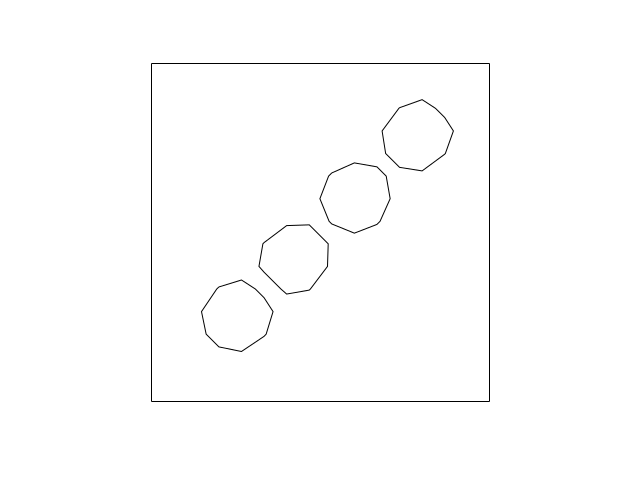
\includegraphics[width=0.98\textwidth]{Figures/cylinderadvection.png}
\end{minipage}
% ---
\begin{minipage}{0.48\textwidth}
\centering
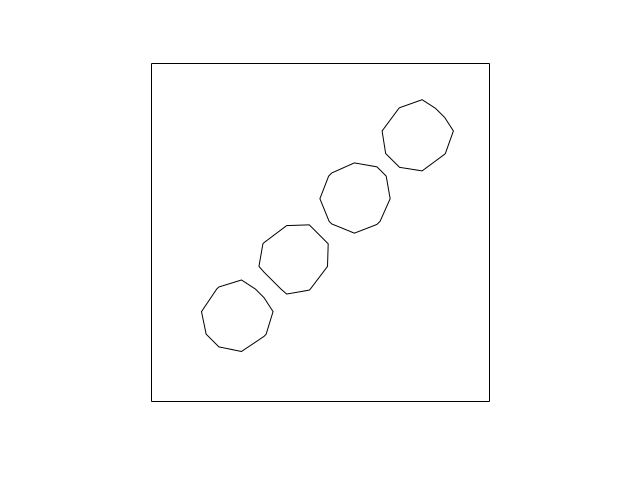
\includegraphics[width=0.98\textwidth]{Figures/cylinderadvectionviscous.png}
\end{minipage}
\caption{Large-density-ratio droplet in a uniform velocity field: a droplet 
with $D/h=3.2$ grid points per diameter is advected in 3D in the plane $z=0$ 
(see text); left:  density ratio $10^9$ without viscosity,
right: density ratio $10^3$ with viscosity}
\label{CylAdv}
\end{figure}
% ----------------------------------------

\subsection{Kelvin Helmholtz Instability}

The Kelvin-Helmholtz instability arises between unequal velocity fluid
streams. It is closely related to the issues addressed in the current
paper since it arises in many of the flows for which the current
method is designed, such as atomisation. Moreover, the
Kelvin-Helmholtz instability is particularly strong on a vortex sheet,
since (as we show below) it has for an infinitely thin sheet a
divergent growth rate as the wavenumber goes to infinity. Compounding
the issue, the baroclinic term of the vorticity equation leads to the
creation of a vortex sheet. In previous papers some of us have studied the
Kelvin-Helmholtz instability in viscous flows with surface tension
\cite{yecko02,boeck05,bague10}

We focus in this paper on the inviscid, no surface tension case since the
objective is to assess the manner in which the advection terms are
treated numerically. Moroever the inviscid, no surface tension case is
a kind of ``worst-case scenario'' without the stabilizing effects of viscosity
and capillarity.

The simplest setup is that of vortex sheeet, for which the growth rate is
given by
\be
\om_i = \frac{2 \sqrt r}{r+1}  k U  \label{omkazi}
\nd




\subsection{Sudden acceleration of a cylinder at large density contrast}

A test that is often included in studies of momentum-conserving methods
\cite{bussmann2002modeling,desjardins10,raessi12,le13,Vaudor:2017ip}
and other methods designed to improve the stability of two-phase flow
computations \cite{Fuster2013energy} is to initialize a droplet of very
high density at velocity $\U_l(\X)=U_0 \E_x$ with the other lighter fluid at
rest, so that $\U_g(\X)=0$. Surface tension and viscosity are not present 
as in the previous test, the only difference being the
discontinuity of the initial velocity on the interface. 
The initial velocity condition amounts to a vortex sheet on the surface 
of the cylinder. After the first time step, the projection method (\ref{fotm}) 
adds a dipole potential flow so that $\U_g = U_0 \E_x + \tau \nabla p / \rho_g$ 
in the gas around the droplet, identical to the dipole flow around a solid object.
However in addition to the dipole flow there could be small multipole components 
to the outer gas flow. 
There are three ways to estimate the perturbations created on the interface.
% ----------------------------------------
\begin{figure}
\begin{center}
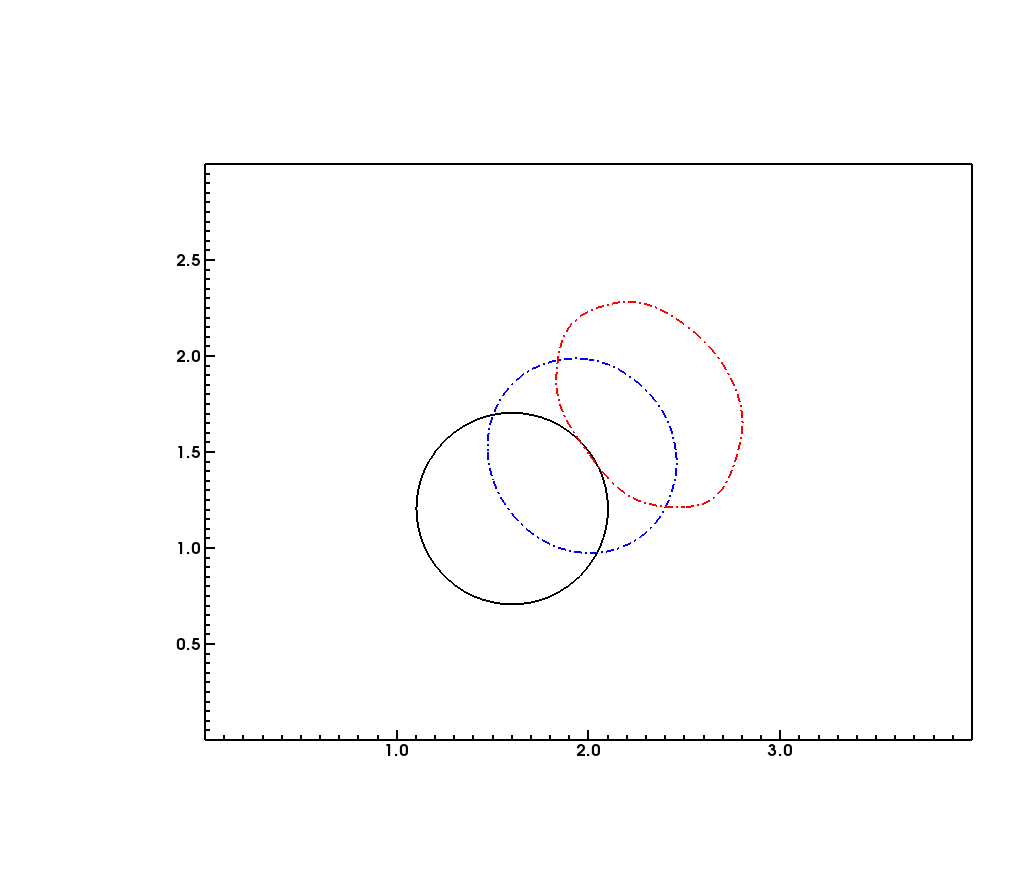
\includegraphics[width=0.4\textwidth]{Figures/Sagar/a.png}
\quad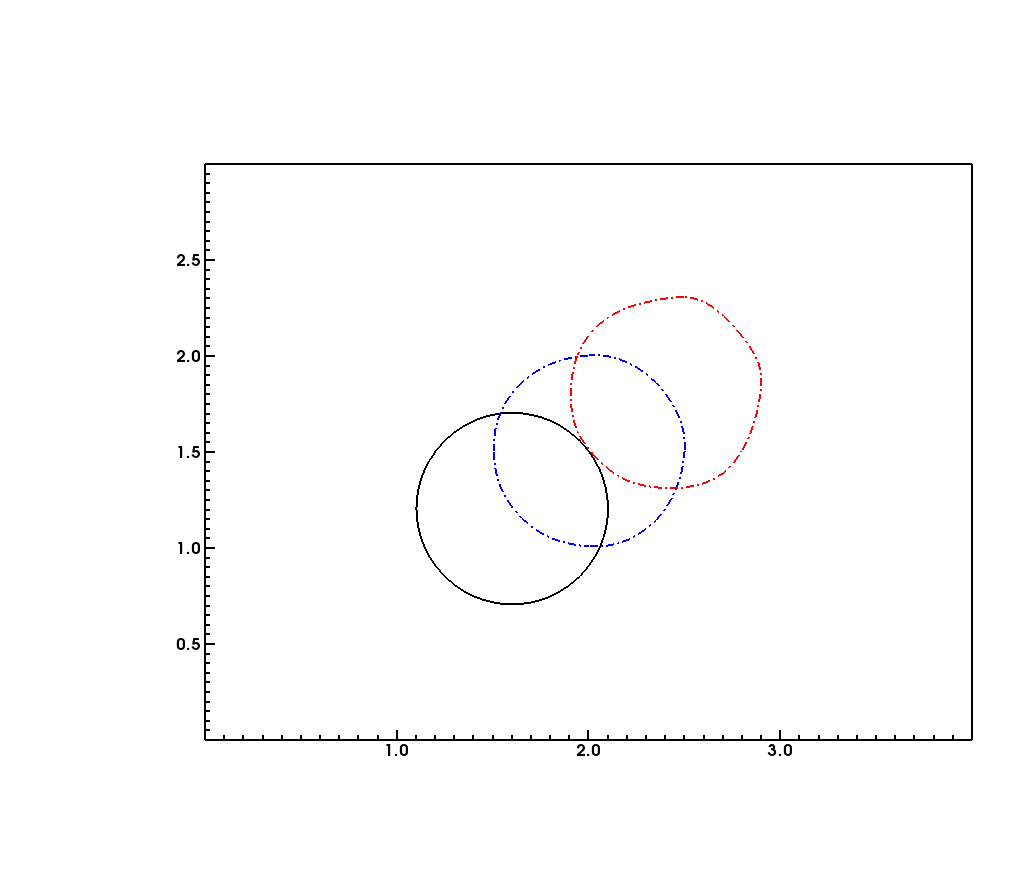
\includegraphics[width=0.4\textwidth]{Figures/Sagar/b.png} \\
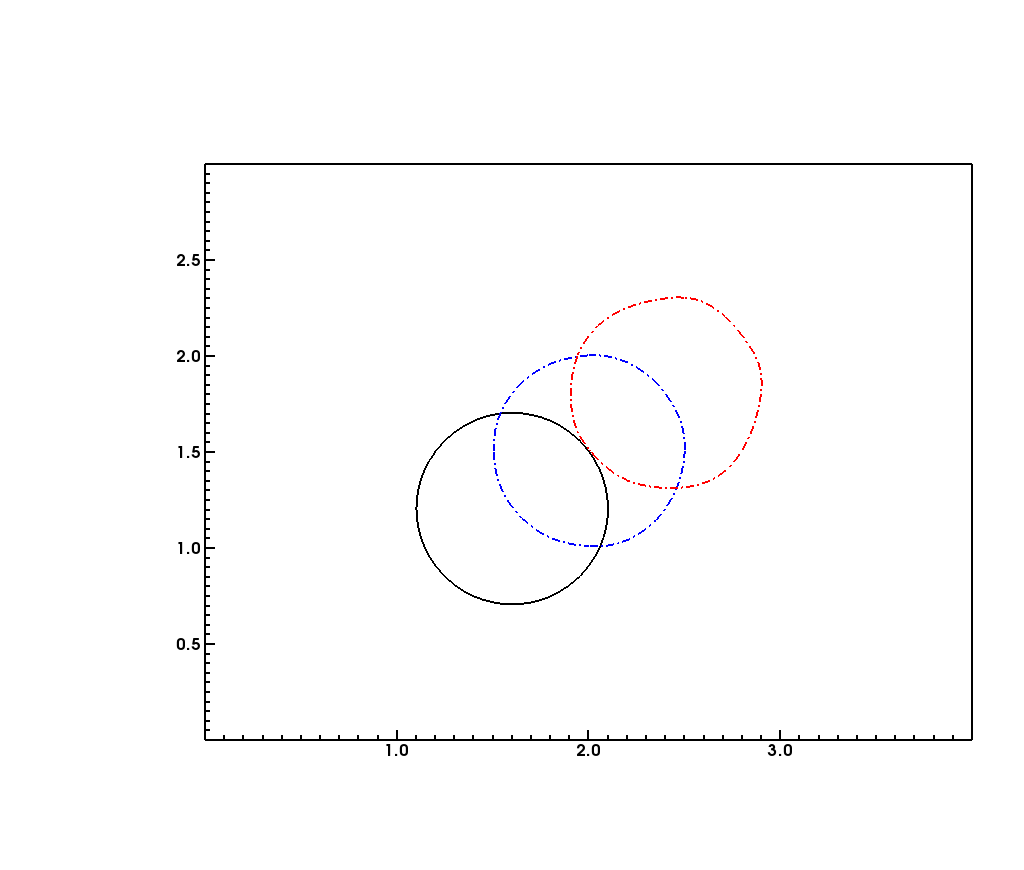
\includegraphics[width=0.4\textwidth]{Figures/Sagar/c.png}
\quad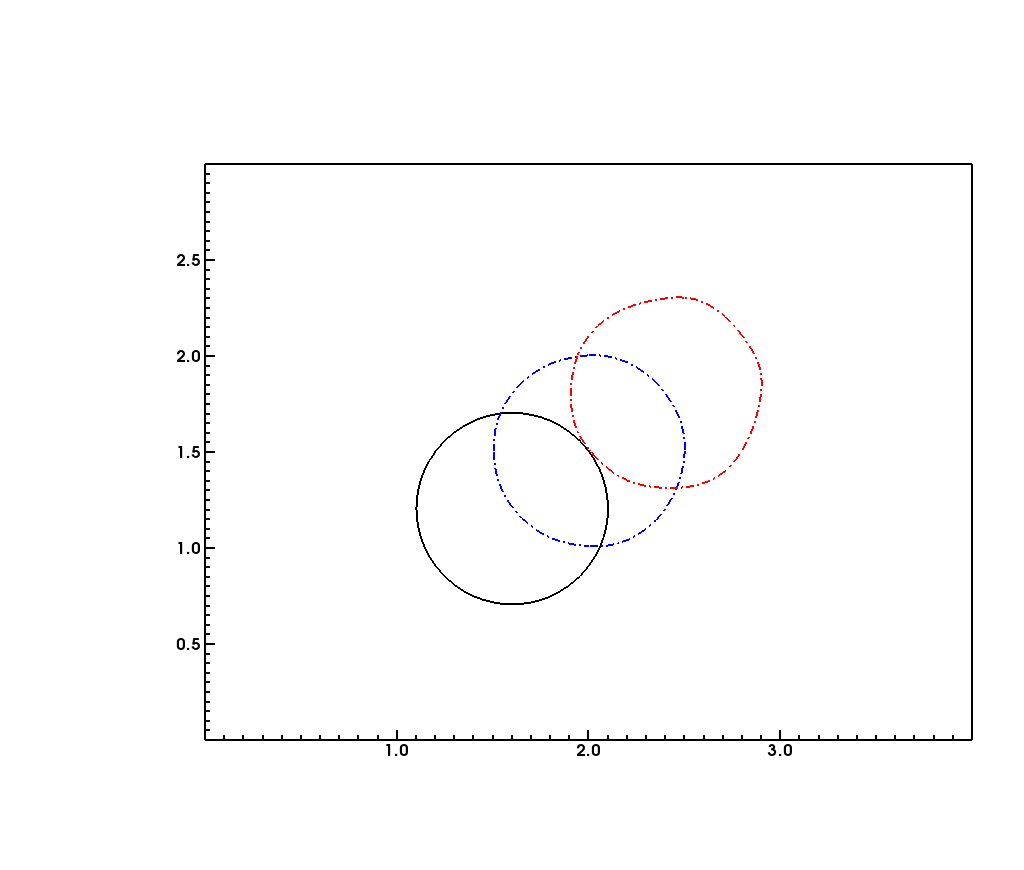
\includegraphics[width=0.4\textwidth]{Figures/Sagar/d.png} \\
\end{center}
\caption{Deformation of a droplet moving through a light fluid. 
From left to right and top to bottom: $r=10,10^3,10^6,10^9$. 
Black shape at $t=0$, blue at $t=D/(2U)$ and red at $t=D/U$. 
The grid resolution is $D/h=20$.}
\label{rich}
\end{figure}
% ----------------------------------------

% ----------------------------------------
\begin{figure}
\begin{center}
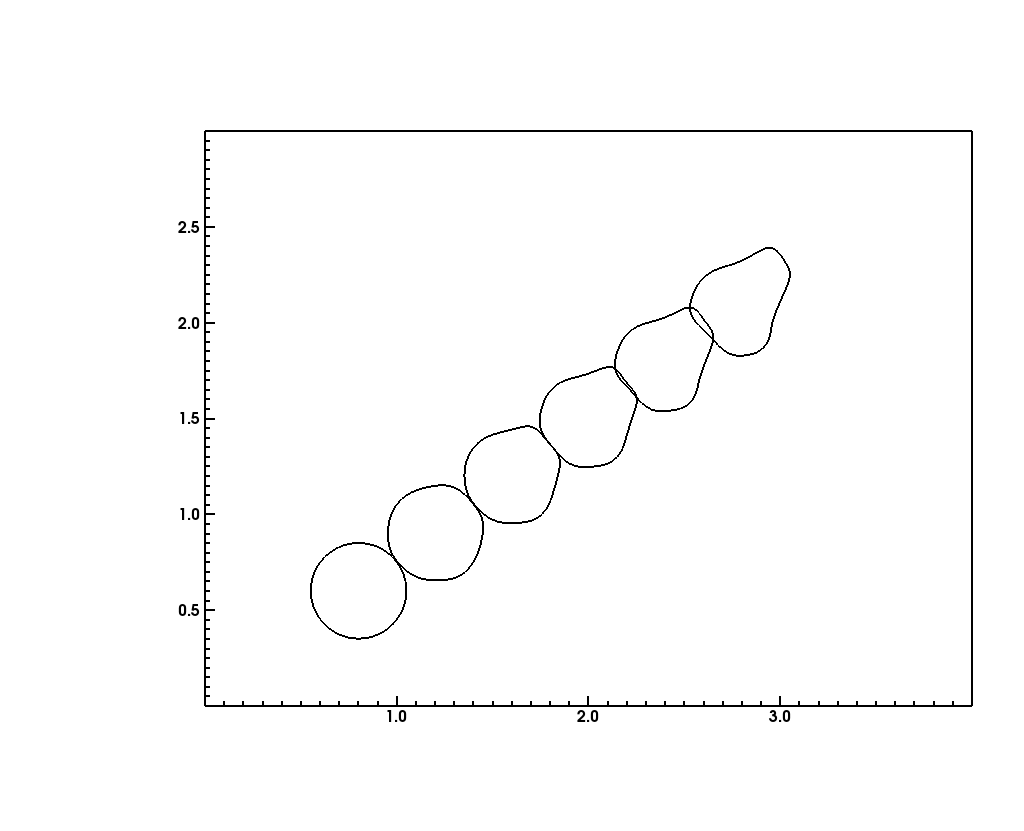
\includegraphics[width=0.4\textwidth]{Figures/Sagar/long.png}
\end{center}
\caption{Deformation of a droplet moving through a light fluid at $r=10^9$.
The grid resolution is $D/h=20$.}
\label{long}
\end{figure}
% ----------------------------------------
A vortex sheet is unstable with respect to the Kelvin-Helmholtz instability. 
The main results about the amplitude of the instability are as follows. 
Let $A(t)$ be the maximum deviation of the interface which has a dimension of length. 
For flows with no viscosity and surface tension
as is the case here, the  Kelvin-Helmholtz instability amplitude $A(t)$  should grow exponentially from a perturbation 
of wavenumber $k$ as $A(t) \sim A(0) \exp ( s_k t )$ with $s_k =| \Delta U | k/ \sqrt r  $ where $ \Delta U $ is
the tangential velocity difference and $r=\rho_l/\rho_g$. In the limit of large $r$ the growth rate becomes small. Since the maximum wavenumber on the grid is $\pi/h$ an estimate of the growth rate of the small wavelength instabilities is $\pi U_0 N/(D \sqrt r)$ where $N$ is the number of grid points per diameter. After advection by a droplet diameter, the 
elapsed time is $\Delta t = D/U_0$. For typical values in the literature of $r=10^6$ and an arbitrary value of 
$N=32$ the amplitude growth would be 
\be
\exp (s_{\rm max} \Delta t) =  \exp\left( \frac{\pi N}{ \sqrt r} \right) 
= \exp ( 0.032\pi) = 1.1058\ldots
\nd
which means the amplitude should grow by 10\% after advection by one diameter 
and by $e^{1/2}$ after the typical advection by 5 diameters. 

Beyond the linear growth stage of the Kelvin-Helmholtz instability, there is a 
self-similar, non-linear growth stage for which dimensional analysis implies
that $A(t) \sim | \Delta U | t/ \sqrt r $ \cite{hoepffner11}. By this argument 
also the perturbation of the cylinder should remain  of order  
$A(\Delta t) \sim D / \sqrt r$ after advection by a droplet diameter. 
One should note that the self-similar growth is obtained for vanishing boundary 
layer thickness but we precisely expect such a velocity discontinuity in 
the present case with no viscosity. 

A final, physical deformation is expected from the spatial pressure variation 
induced by the dipole gas flow. This variation involves a larger pressure at 
the aft and fore stagnation points and a lower pressure along the ``equator'' 
of the droplet \cite{Clift78}. The resulting integrated stress is of order 
$\rho_g U^2$ resulting in the growth of the droplet deformation as 
$A(t) \sim U^2 t^2 / (D r)$ and after advection by a droplet diameter as
$A(\Delta t) \sim D / r$. 
This growth is observed experimentally \cite{opfer14} and results in an 
elliptically shaped drop, albeit of much smaller amplitude than the two former 
Kelvin-Helmholtz-related growth mechanisms. 

The results are shown on Figure \ref{rich} for several times and
density ratios in a manner comparable to \cite{bussmann2002modeling}. For these
numerical experiments, the exact manner of initializing the velocity fields has 
some importance. It is important not to allow in the first time step some gas 
velocity in the liquid to avoid large pressure gradients in the liquid. 
Thus the density is initialized to $\rho_l$ to machine accuracy using the 
{\sc Vofi} library \cite{bna2015numerical,bna2016vofi}
within a disk implicitly defined by $x^2 + y^2 + z^2 < R^2$ 
and the velocity is initialized to 1 for all the velocity nodes inside
a disk implicitly defined  by  $x^2 + y^2 + z^2 < (R+nh)^2$, where $n$ is the 
size of the ``halo'' in number of grid points. The velocity in the other
nodes is initialized to 0. The tests shown were performed with $n=1$. 
Increasing the size of the halo from $n=0$ to $n=1$ improves the results in the 
first phase of the droplet motion, but not in the late phase. 

The velocity of the motion has been oriented on the diagonal as in 
\cite{bussmann2002modeling}. The WY scheme is used with a QUICK
interpolant. The droplet deforms little after advection by one droplet 
diameter (Figure \ref{rich}). For longer advection the deformation is worse 
but, as explained above, this is to be expected
at high resolution, except in the $r=10^9$ case for which we show advection 
by 5 diameters in Figure \ref{long}. 
If the non-momentum-conserving method is used, the
droplet deforms rapidly and the simulation breaks down. As expected
the results are better than those of \cite{Fuster2013energy}, that uses the
skew-symmetric scheme but without momentum-conserving-like schemes, 
but worse than those of \cite{bussmann2002modeling,desjardins10,raessi12,le13}. 
It is also seen, as expected from the developments above, 
but perhaps contrary to intuition, that it is easier
to have larger density contrasts. Increasing the number of grid points also helps.


A comment can be made on the nature of the instabilities seen. If
 the gas velocity numerically diffuses inside the liquid, then some vorticity
may penetrate into the liquid despite the fact that in inviscid flow
vorticity should remain confined on the interface. If this happens,
the growth rate of a single-phase Kelvin-Helmholtz instability inside the 
liquid is the much larger value $\widetilde{s}_k =| \Delta U | k/2$, 
without the $\sqrt r$ factor at denominator. \red{(The derivation of this fact 
may be found for example in \cite{matas2011experimental}.)} 
The instability seen for the $r=10^9$ case for the long advection case in  Figure \ref{long} is 
a mode 3, which excludes the large linear growth discussed above for small 
wavelenghts rather points to the velocity diffusion mechanism. 
Minimizing numerical diffusion should then be an important
quality for this test, while on the other hand numerical diffusion may
stabilize other difficult test cases/situations. 

\red{
\subsection{Sheared layer}
In order to better analyze the behavior of the methods in flow under shear, 
such as vortex sheets and Kelvin Helmholtz instabilities, we setup directly 
a planar, parallel shear flow in a $(-1/2,1/2)^2$ domain with the following 
initial condition
\bea
u_1& = 15 &\qquad {\rm if \;\;} |x_2| > 1/10 \nonumber \\
u_1& = 1  &\qquad {\rm if \;\;} |x_2| < 1/10 \nonumber 
\nda
$$
u_2  =  0.01\, \sin(2 \pi x_1) \exp(-20 x_2^2)
$$
and $\rho=1$  if $|x_2| > 1/10$ and $\rho=10^3$ otherwise. 
This flow is similar to a liquid sheet in high velocity gas. The flow is 
simulated until time $t_f=2$ unless the simulation blows up at an earlier time
$t_b <t_f$.
Table \ref{shearmtable} shows the numerical schemes that have been used in a few
simulations together with the fraction $t_{b}/t_f$ of the final time that has 
been reached. All simulations have been performed on a $128\times128$ grid with 
a CFL of 0.03 and a density ratio of 1000. The new method (MC) is
systematically more stable than the standard method for the two combinations 
shown in Table \ref{shearmtable}: a) the WY VOF scheme and the QUICK-UW velocity 
interpolation schemes and b) the CIAM VOF with the Superbee slope limiters. 
The state of the two simulations with the first combination of schemes is shown
in Figure~\ref{shelay}, just before breakdown at time $t_b = 0.34$ 
(or $t_b/t_f = 0.17$) for the (MC) method, and at time  $t_b = 0.16$ 
(or $t_b/t_f = 0.08$) for the standard method. We have also tested a number of other
combinations, for example  WY \& Superbee that turns out to be very unstable.  
We have also performed simulations with smaller  $64\times64$ and $32\times32$ 
grids that yield similar results. 
Finally, we note that this case is also unstable in a single-phase configuration 
when using the QUICK third-order velocity interpolation.
% -----
\begin{table}
\input notes
\caption{Percentage of completion of the shear layer test with various methods. 
All simulations are performed on a $128\times128$ grid with a CFL of 0.03 
and a density ratio of 1000.}
\label{shearmtable}
\end{table}
% -----

% -----
\begin{figure}
\begin{center}
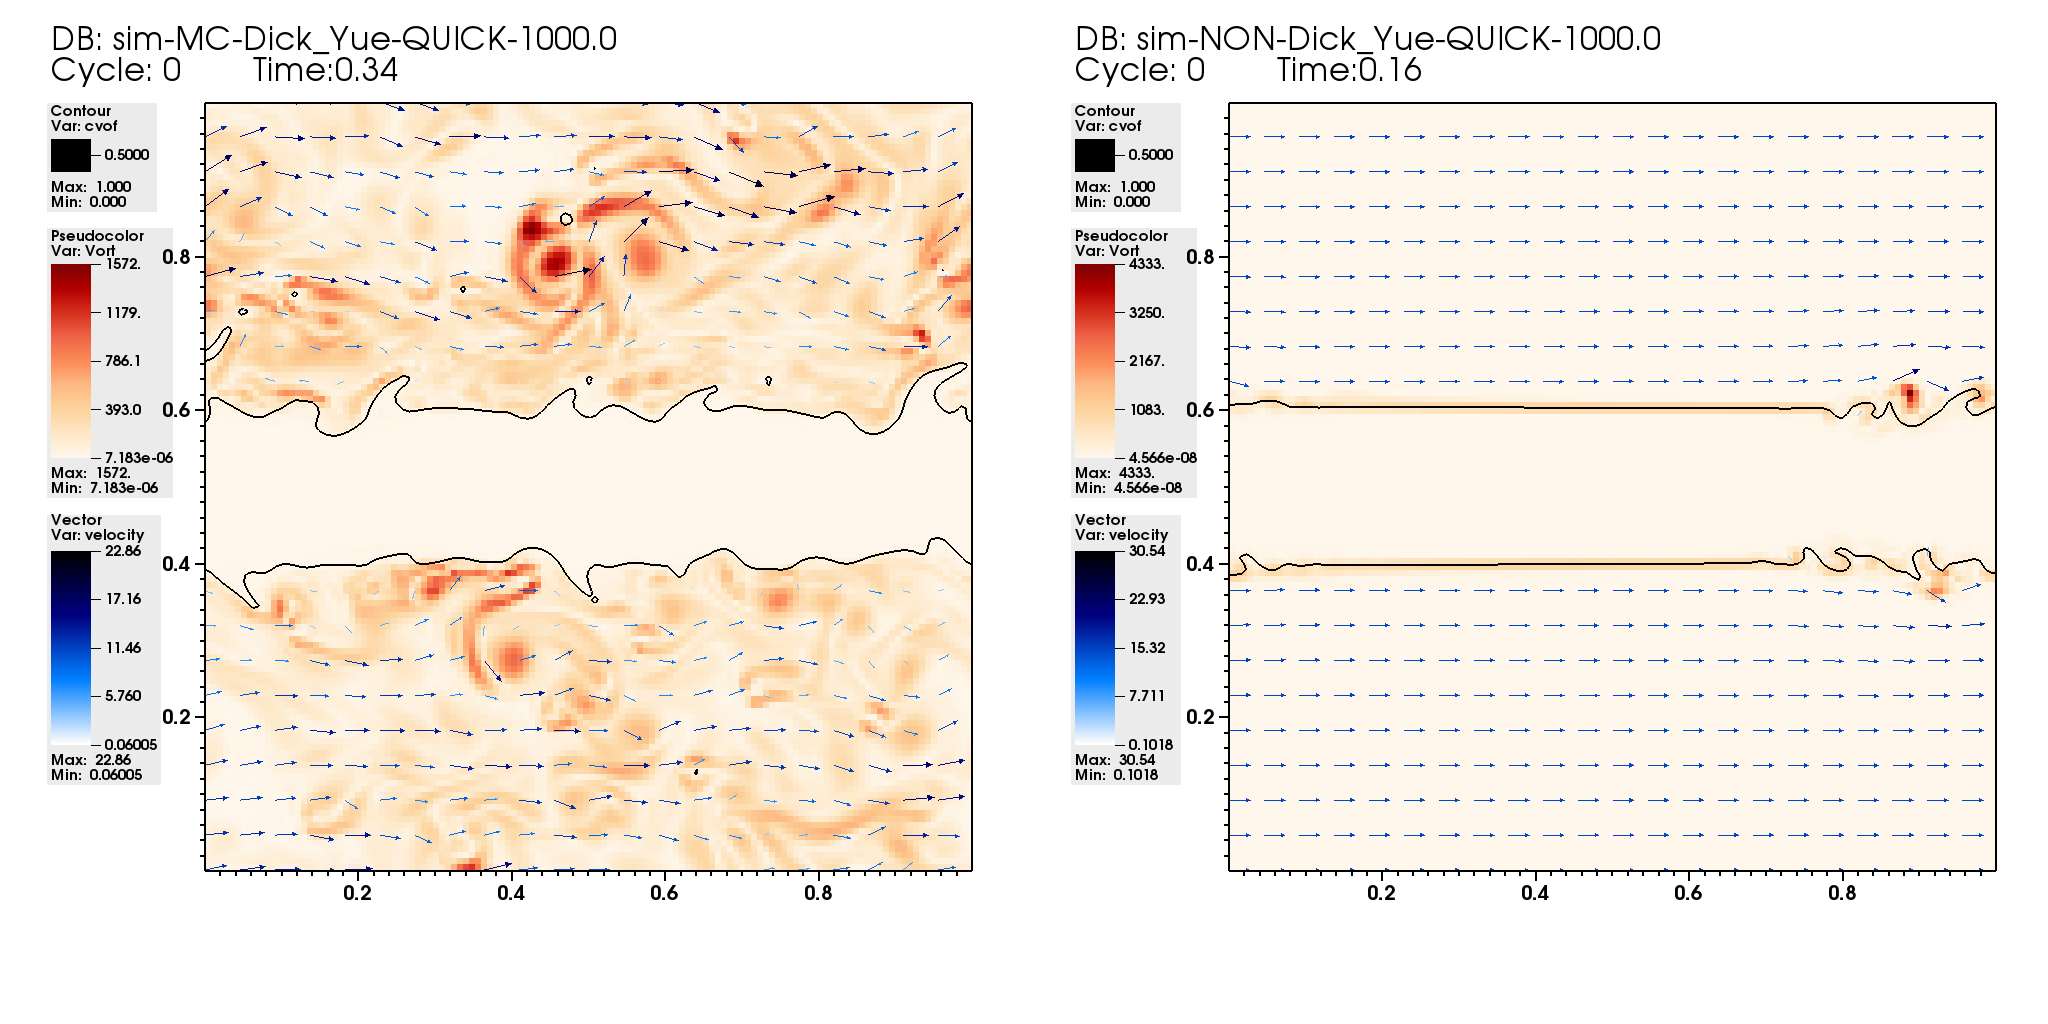
\includegraphics[width=\textwidth]{Figures/Sagar/shear.png}
\end{center}
\caption{The state of the simulation of the sheared layer just before eventual 
breakdown of the simulation with the combination of WY VOF scheme
and QUICK-UW interpolation. Left: (MC) method, right: standard method.}
\label{shelay}
\end{figure}
% -----
} 
% end red section

\subsection{Falling Raindrop}
% Basic setup 

A flow configuration that combines the complexities of high density-ratios with the interaction between capillary, viscous and inertial stresses is that of a water droplet falling in air under the influence of gravitational acceleration. The problem is characterized by a combination of Reynolds, Weber and Bond numbers, the definitions of which are as follows : 

\begin{align}
We=\frac{\rho_{\rm air} U^2 d}{\sigma} \quad,\quad Re= \frac{\rho_{\rm air} U d}{\mu_{\rm air}} \quad,\quad Bo=\frac{\left(\rho_{\rm water}-\rho_{\rm air}\right) g d^2 }{\sigma}
\end{align}

\vspace*{0.2cm}

In our particular numerical setup, $We \simeq 3.2 $, $Re \simeq 1455 $ and $Bo \simeq 1.0 $, thus corresponding to that of a $3mm$ diameter raindrop (a relatively large one) falling in air at an approximate terminal velocity of  $8$ m/s (interpolated from empirical data, refer to  \cite{gunn1949terminal}). The parameters in the problem setup is given in Table \ref{raindropprop}, and the schematic diagram given by Fig. \ref{setup}. The droplet is initially placed at the center of a cubic domain (3D), whose side is 4 times the diameter of the drop. 

\vspace*{0.2cm}

% -----
\begin{table}[h!]
\begin{center}
\begin{tabular}{ccccccc}
\hline\hline
$\rho_{\rm air}$ & $\rho_{\rm water}$ & $\mu_{\rm air}$ 
& $\mu_{\rm water}$ & $\sigma$ & $d$ & $g$\\
$\left(kg/m^3\right)$ & $\left(kg/m^3\right)$ & $\left(Pa \, s\right)$ 
& $\left(Pa \,s \right)$ & $\left(N/m\right)$ & $(m)$ & $(m /s^{2})$ \\
\hline
1.2 & $0.9982 \times 10^3$ & $1.98 \times 10^{-5}$ & 
$8.9 \times 10^{-4}$ & $0.0728$ & $3 \times 10^{-3}$ & $9.81$\\
\hline\hline
\end{tabular}
\caption{Parameter values used in the simulation of a falling water droplet in air. \label{raindropprop}}
\end{center}
\end{table}
% -----

\vspace*{0.2cm}

In order to properly reproduce and analyse the dynamics of a relatively large drop (high Reynolds flow) such as in our case, the numerical method has to accurately resolve the thin, complicated boundary layers, the interaction of such layers with the capillary deformations and finally the non-linear feedback of the complex 3D vortical structures in the droplet wake to the surrounding pressure field. Therefore, we explicitly state that the aim of this particular test case is not to develop a high fidelity model of a raindrop, but rather carry out a stringent evaluation of the robustness of our numerical method compared to methods which are not momentum consistent. For such a low Weber number the capillary forces dominate and the droplet should remain approximately spherical, and should definitely not undergoe any subsequent atomization. 


% -----
\begin{figure}[h!]
\begin{center}
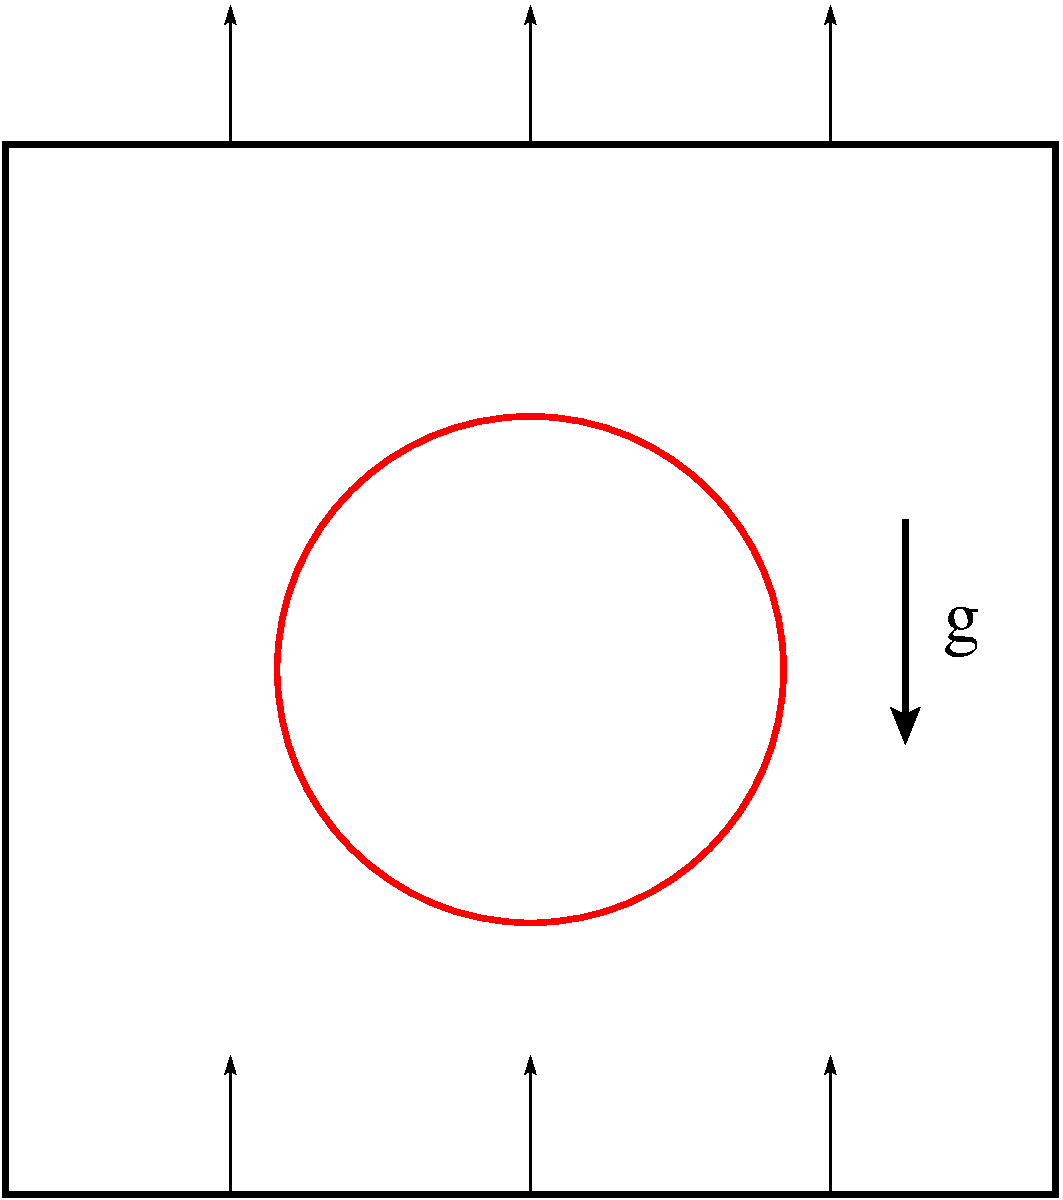
\includegraphics[width=0.35\textwidth]{Figures/setup.pdf}
\end{center}
\caption{Problem setup for falling rain drop test case. Boundary conditions 
at the top and bottom are a uniform inflow and outflow velocity $U_0(t)$. 
Boundary conditions on the side are free slip (no shear stress).}
\label{setup}
\end{figure}
% -----


% -----
\begin{figure}
\begin{center}
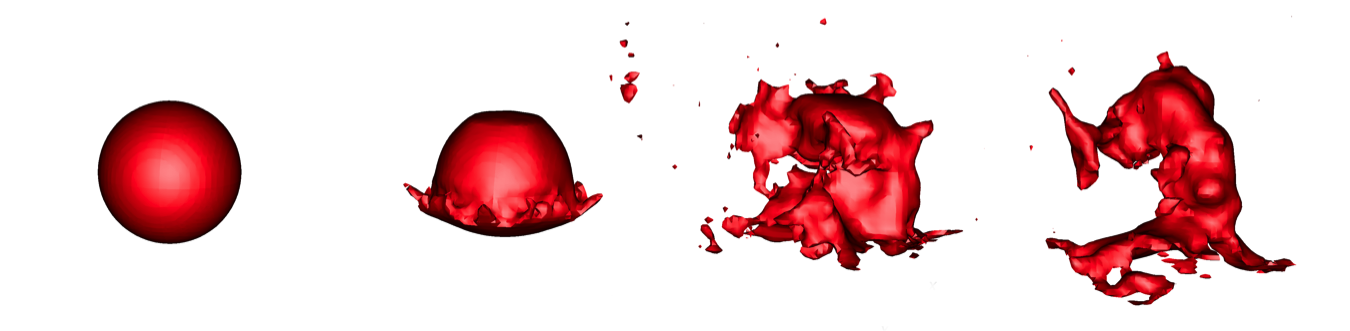
\includegraphics[width=0.75\textwidth]{Figures/cata.png}
\end{center}
\caption{Rain drop test case: catastrophic breakup with non-conserving 
formulation, $D/h=30$.}
\label{cata}
\end{figure}
% -----

Numerical simulations of this test case at moderate resolution ($D/h=16$ to 64 grid points per diameter were tested) without the consistent momentum-conserving scheme described in this paper, results in the catastrophic deformations of the droplet as shown in Fig. \ref{cata}, which we like to describe as 'fictitious' or 'artificial' atomization as a result of rapidly growing numerical instabilities. This effect was previously uncovered by \cite{Xiao:2014vs} in a similar case involcing the sudden interaction of a droplet at rest with a uniform gas flow. The Weber number in that case was also approximately 3, therefore one would expect a nearly spherical droplet shape, but the authors of ref. \cite{Xiao:2014vs} have reported a similar catastrophic deformation, forwarding the following explanation. To start with, we neglect gravity and viscous effects at this relatively large Reynolds number. Also, we are interested in steady-state flow. On the axis and near the hyperbolic stagnation point at the front of the droplet one has $u_2=0$ for the transverse (radial) velocity and for the axial momentum balance

\be
u_1 \partial_1 u_1 = - \frac 1 \rho \partial_1 p.
\nd

Because of the low viscosity and large density ratio, it is not possible for the air flow to immediately entrain the water, so the fluid velocity is significantly smaller in the water. In the air the acceleration near the stagnation point is of the order $U^2/D$, whereas the pressure gradient is

\be
\partial_1 p \sim \rho_{a} U^2/D.
\nd
The pressure gradient in the water is much smaller, however in the case of a mixed cell the water density multiplies the air acceleration $U^2/D$, so that
\be
\partial_1 p \sim \rho_{w} U^2/D,
\nd

then a large pressure gradient results in the mixed cell or cells. This large pressure gradient results in a large pressure inside the droplet near the front stagnation point, as shown in Figure \ref{FengXiao}. This large pressure is balanced by surface tension only for a sufficiently large curvature near the droplet front. This explains the presence of a ``dimple'' often observed in low resolution simulations of the falling drop. 

% -----
\begin{figure}
\begin{center}
\begin{tabular}{cc}
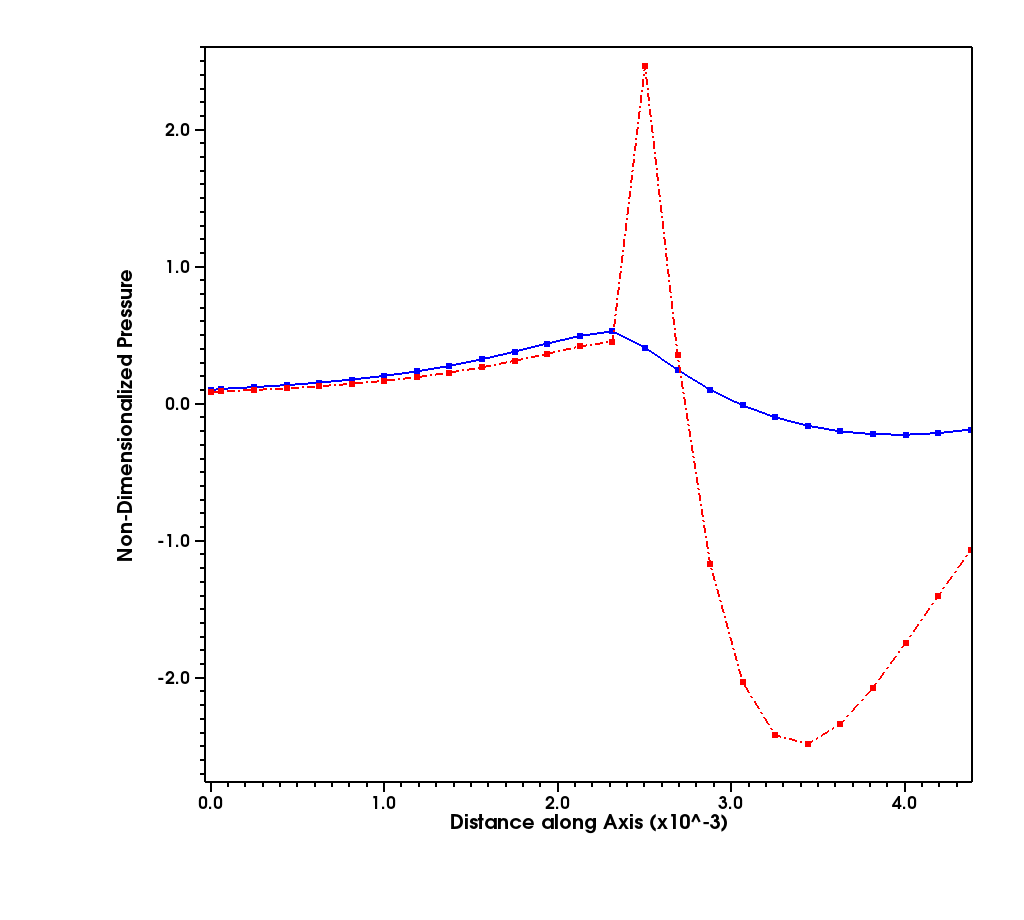
\includegraphics[width=0.45\textwidth]{Figures/Sagar/16ppd_MC_vc_NON-MC.png} &
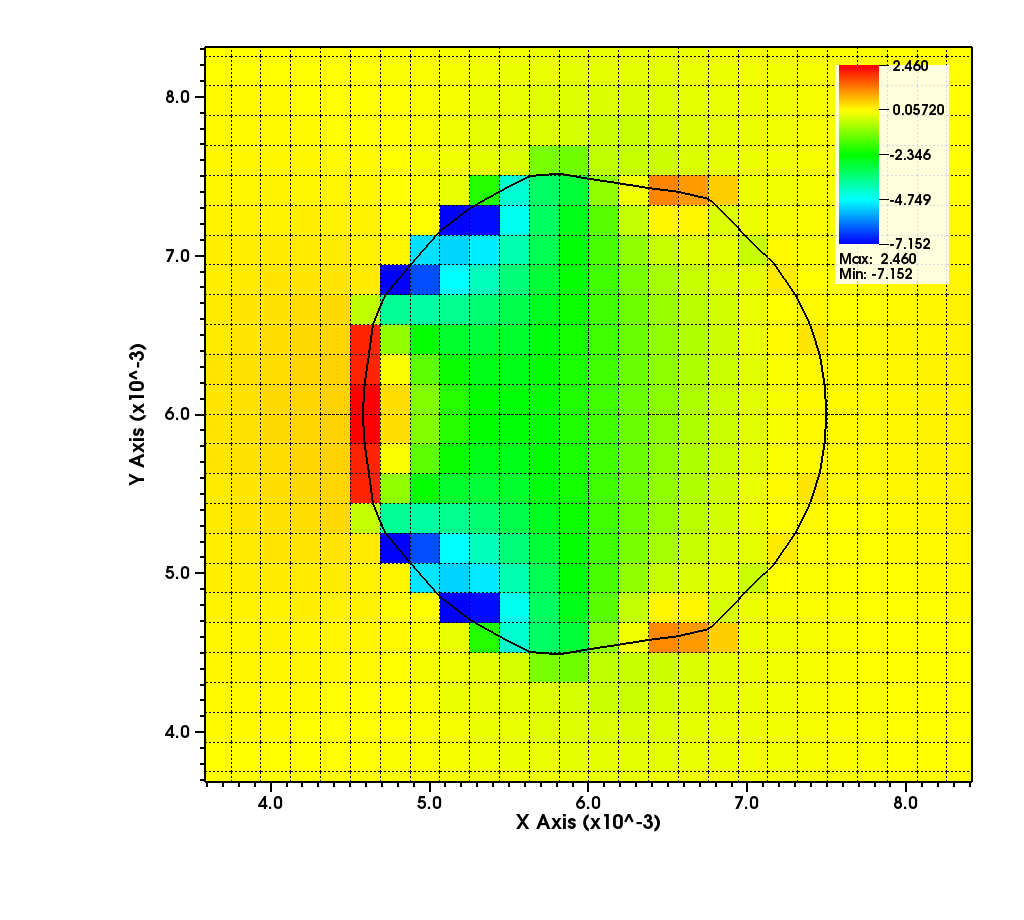
\includegraphics[width=0.45\textwidth]
{Figures/Sagar/non_MC_16ppd_pressure_corrected.png}\\
(a) & (b)
\end{tabular}
\end{center}
\caption{The origin of the pressure peak in the front of the droplet. 
(a) The profile of the pressure on the axis a few timesteps after initialisation 
with the standard, non-momentum conserving method (red) and the present method 
(blue). (b) The pressure distribution immediately after the start of the simulation 
using the standard, non-momentum-conserving method. The pressure peak does
not result yet in the formation of a dimple. In all figures  $D/h = 16$.}
\label{FengXiao}
\end{figure}
% -----

% -----
\begin{figure}
\begin{center}
\begin{tabular}{cc}
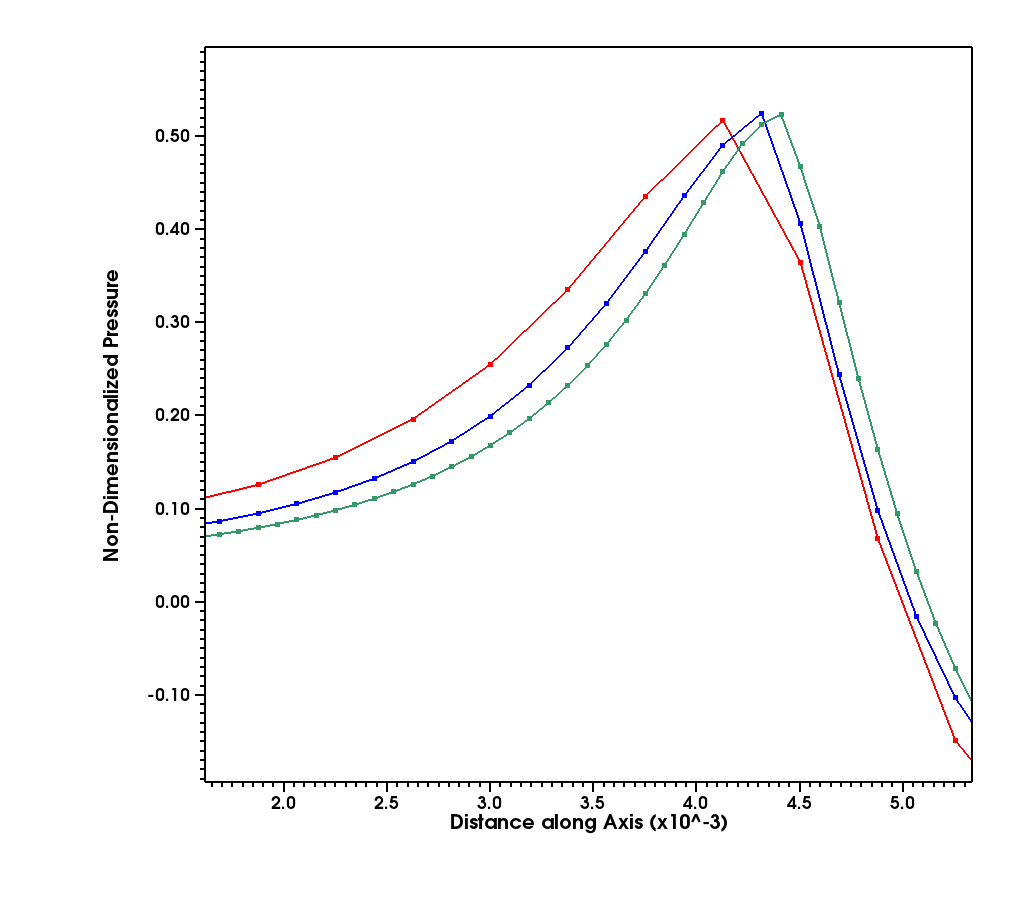
\includegraphics[width=0.45\textwidth]{Figures/Sagar/pressure_rd_MC.png} &
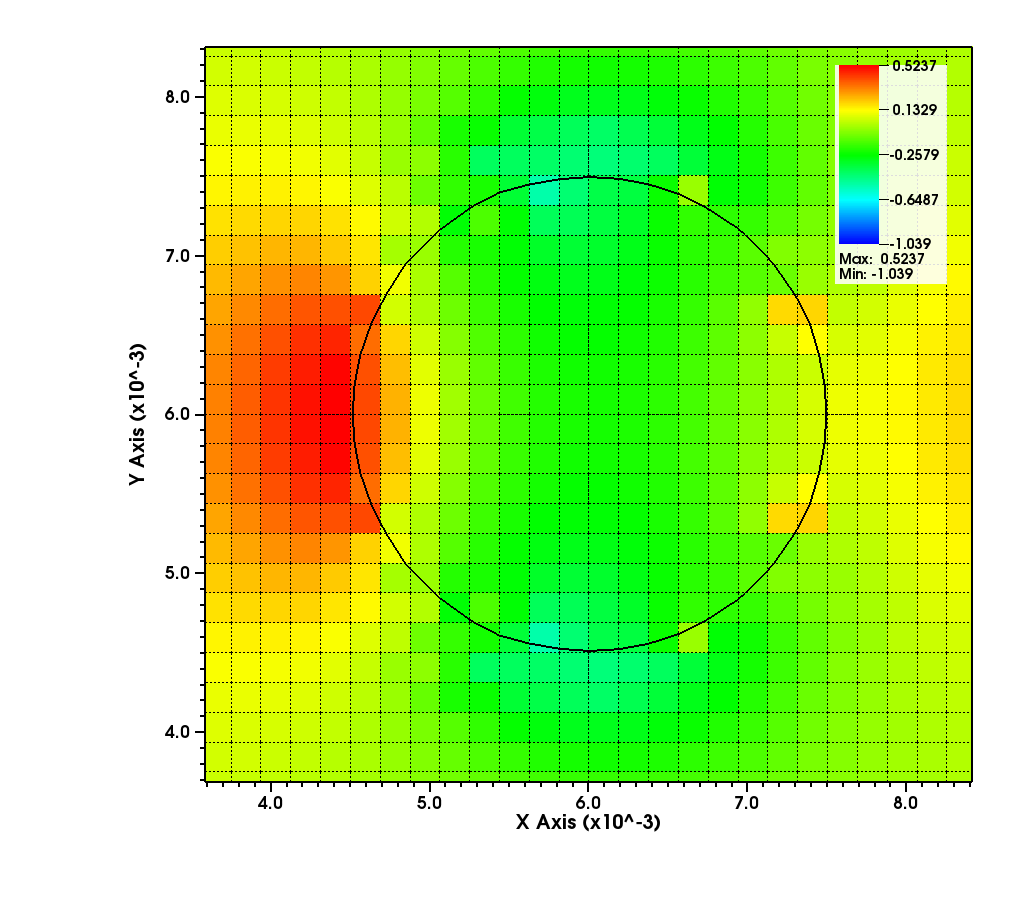
\includegraphics[width=0.45\textwidth]
{Figures/Sagar/16ppd_pressure_corrected.png}\\
(a) & (b)
\end{tabular}
\end{center}
\caption{ (a) The pressure profile on the axis a few timesteps after 
initialisation with the present 
method at various resolutions: $D/h = 8$ (red) , $16$ (blue) and $32$ (green). 
(b) The pressure distribution immediately after the start of the simulation 
using the present method and   $D/h = 16$.}
\label{FengXiao_corrected}
\end{figure}
% -----

\vspace*{0.2cm}

\begin{figure}[!h]
\begin{center}
\begin{tabular}{cc}
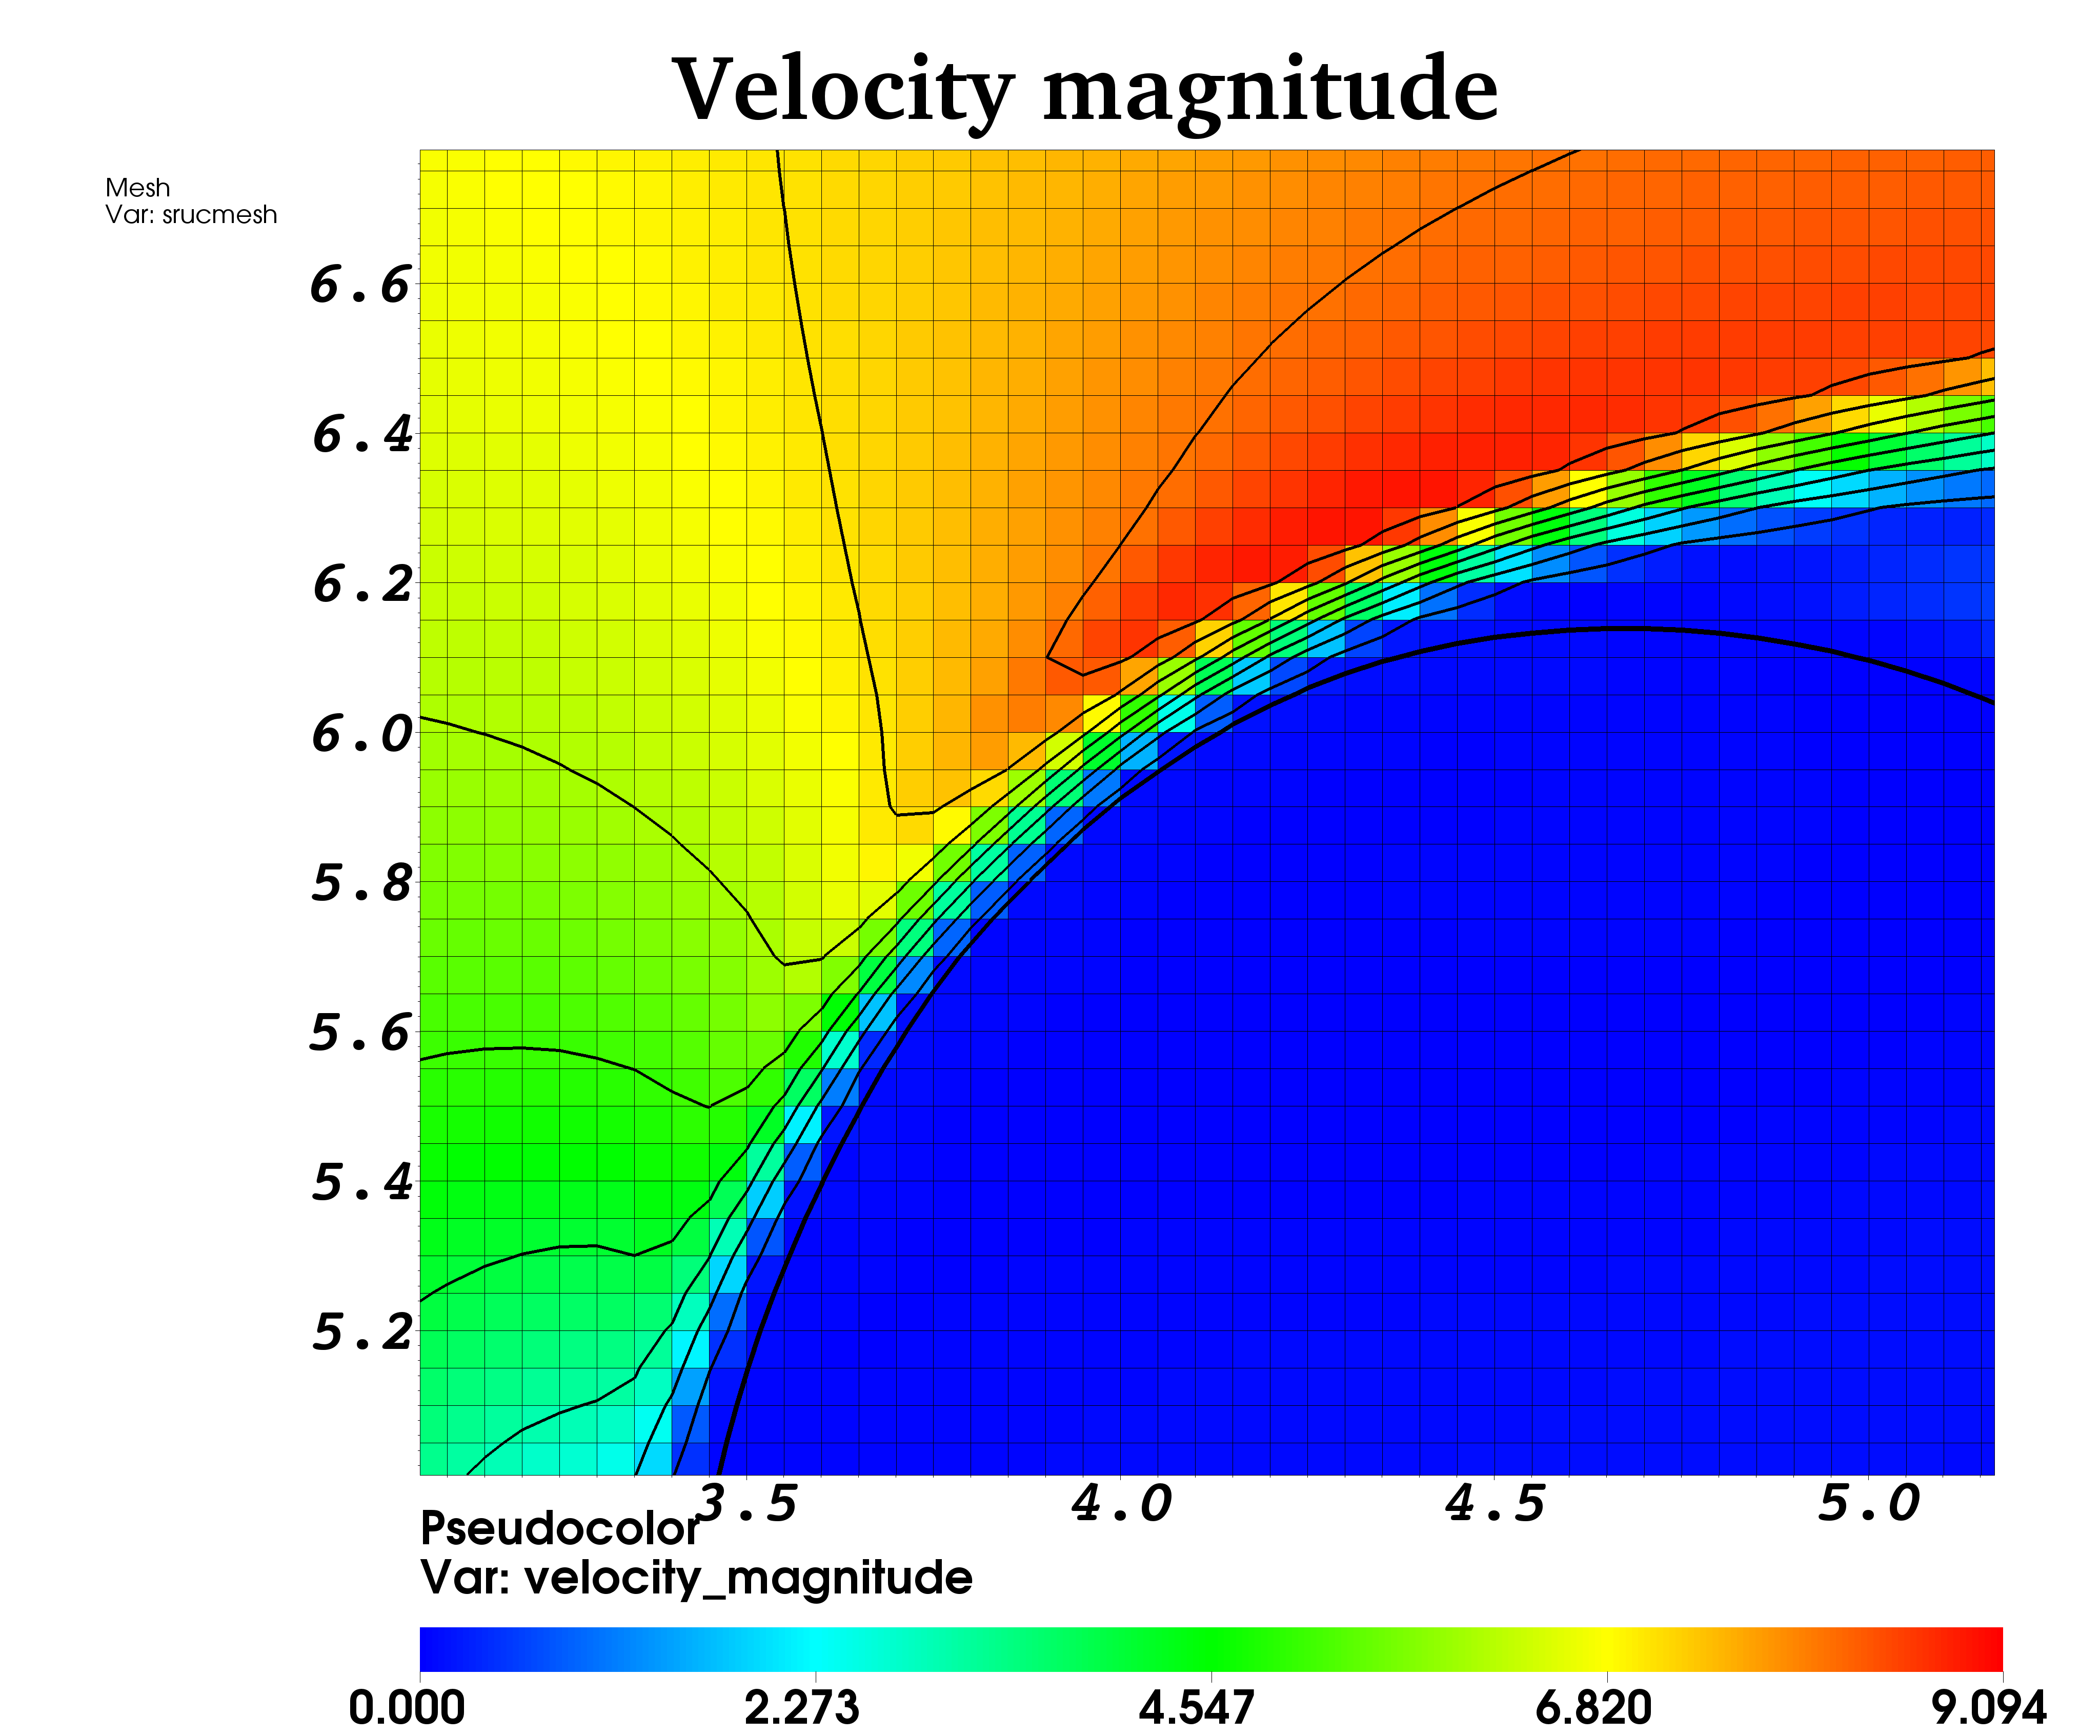
\includegraphics[width=0.42\textwidth]{Figures/vel.png}
& 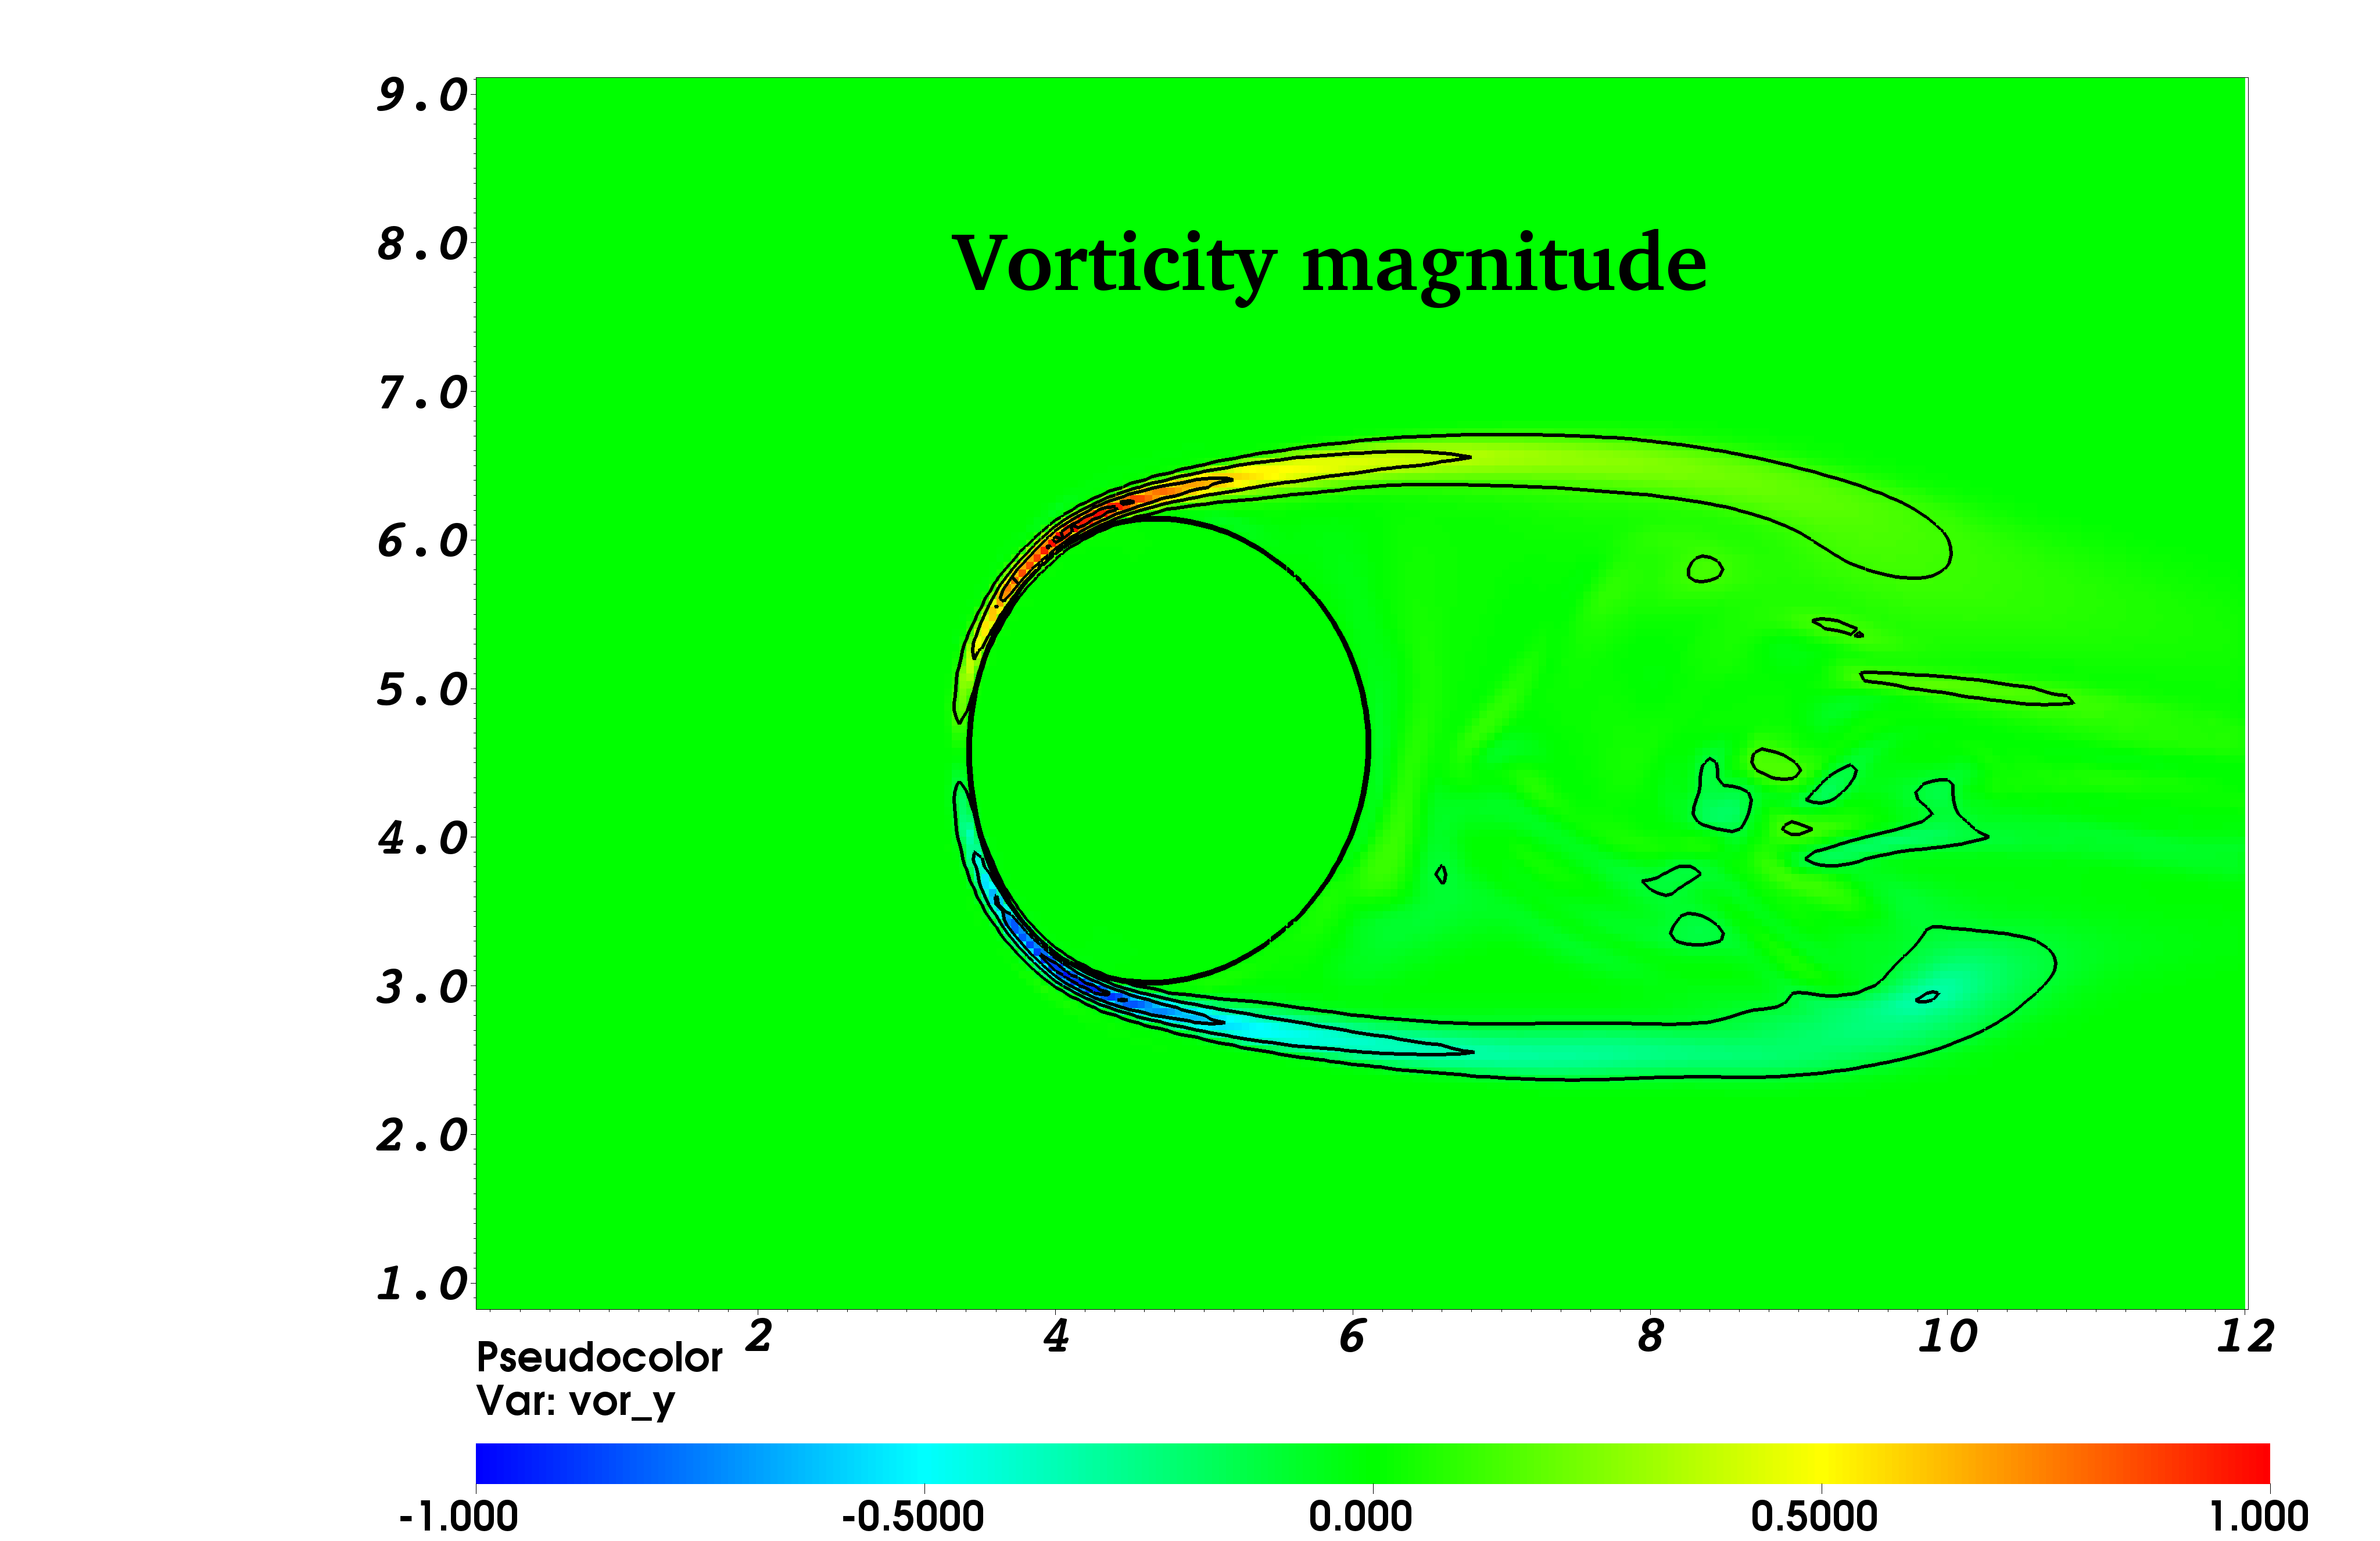
\includegraphics[width=0.48\textwidth]{Figures/vort.png} \\
(a) & (b)
\end{tabular}
\end{center}
\caption{Flow field around the 3 mm droplet with 60 grid points per diameter. 
(a) The velocity magnitude. It is seen that even at this highest resolution 
there are only three points in the boundary layer. (b) The vorticity magnitude. 
The marked separation of the boundary layers is observed with 
a more complex vortical region in the wake.}
\label{magn}
\end{figure}
% -----
\newcommand\DDD{{\cal D}}

Visualization of the flow around the droplets (Figure \ref{magn}) illustrates the challenging nature of the flow configuration, even for such a seemingly simple physical problem. As one can observe, the boundary layers are extremely thin, hence questioning our approximation that fluid velocity is continuous across the interface. We observe that applying the numerical method described in this paper brings a considerable and systematic improvement over a range of different flux limiters (WENO, ENO, Superbee, QUICK, Verstappen) and CFL numbers, as evidenced by comparing the figures \ref{FengXiao} and \ref{FengXiao_corrected}. To summarize, the simulations broadly fall in three categories: 

\begin{enumerate}
	\item They blow up anyway even while applying the present method
	\item They keep physical values of the kinetic energy and smooth interfacial shapes.
	\item They have a marked peak in kinetic energy as a function of time, associated with massively deformed interface shapes, 
\end{enumerate}

Regarding the first two points made above, we find that certain combinations of the advection scheme (CIAM/WY) and the flux limiter (ENO/WENO/Superbee/Verstappen/QUICK) display more numerical stability that the others, in particular, the most stable combinations of schemes are CIAM advection with Superbee limiter and the WY advection with QUICK limiter. As a minor remark, the CIAM advection with the Superbee limiter also appears to be quite diffusive. The third point highlights the systematic behavior of the simulations that are carried out without applying the present momentum-conserving method. 

\vspace*{0.2cm}

\begin{figure}[h!]
\begin{center}
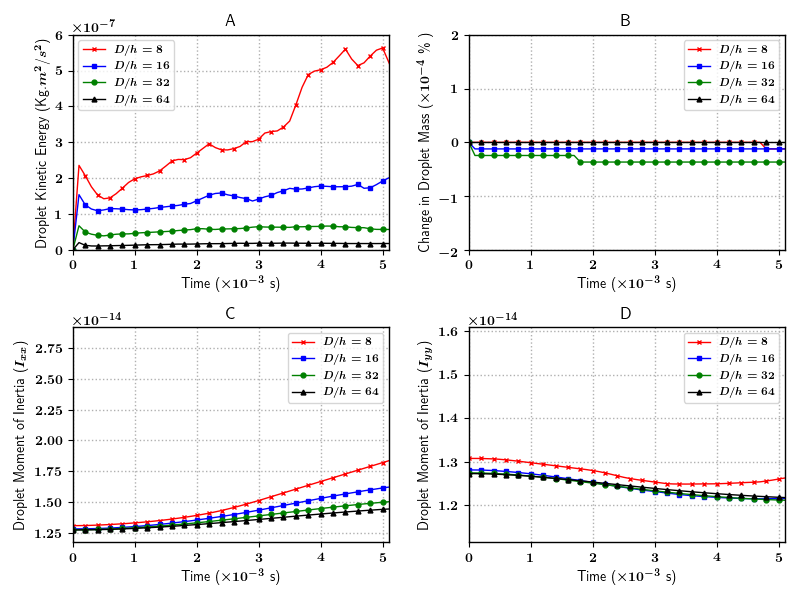
\includegraphics[scale = 0.6]{Figures/Sagar/multiplot_raindrop.png}
\end{center}
\vspace*{-0.5cm}
	\caption{Temporal evolution of quantities of interest to evaluate the performance of our present method for different spatial resolutions. (A) Kinetic energy of the droplet. (B) Percentage change in the droplet mass from initialized mass. (C) Moment of inertia of the droplet along flow (X) direction. (D) Moment of inertia of the droplet along direction perpendicular to flow (Y,Z), evolution of $I_{yy}$ is identical to $I_{zz}$, thus the latter is not shown.}
\label{multi}
\end{figure}

We illustrate the performance of the present method through the results of our simulations in Figure \ref{multi}. We have carried out simulations corresponding to $D/h = 8, 16, 32 $ and $64$, while keeping the same value for the inflow velocity boundary condition. The quantities of interest while examining the robustness of the method are the temporal evolution of the droplet kinetic energy (Fig. \ref{multi}. A) and droplet mass (Fig. \ref{multi}. B), as well as moment of inertia of the droplet along directions aligned to the inflow velocity (Fig. \ref{multi}. C) and orthogonal (Fig. \ref{multi}. D) to it. The moment of inertia is used as a descriptor of the 'average' droplet shape, with the three moments of inertia along the different axes $I_m$ defined as - 

\be
I_m = \int_\DDD H x_m^2 {\rm d}\X \;, \quad  1 \le m \le 3,
\nd

where $\DDD$ is the computational domain and $x_m$ is the distance of the interface relative to the center of mass of the droplet.   

\begin{figure}[h!]
\begin{center}
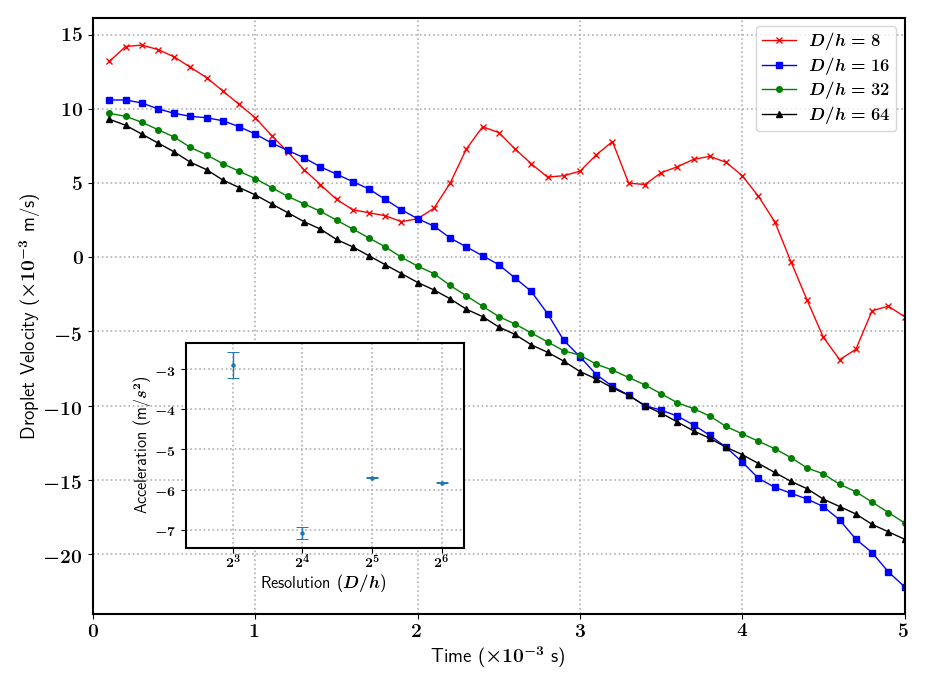
\includegraphics[scale = 0.5]{Figures/Sagar/dropl_velocity_accel_ppd.png}
\end{center}
\vspace*{-0.5cm}
\caption{Comparison of droplet velocity as a function of time, for different droplet resolutions, The droplet velocities correspond to that of their respective center of masses. Inset : Convergence of the droplet acceleration as a function of resolution, computed using the best linear fit over the temporal variation of their respective velocities. The error bars signify the asymptotic standard error (least-squares) corresponding to the obtained linear fits.} 
\label{drop_vel}
\end{figure}

The kinetic energy of the droplet evolves in a relatively smooth manner, without the presence of sudden spikes and falls which are emblematic of the non-conservative version of our method. Such abrupt changes in kinetic energy of the droplet have been found to be associated with instants when the droplet undergoes 'artificial' atomization or breakup, henceforth resulting in the catastrophic loss of stability for the numerical method. We observe a systematic drop in the amount of the droplet kinetic energy as we increase resolution, with the most probable explanation being that of the suppression of spurious interfacial oscillations which are rampant at low resolutions. There is also a component of the kinetic energy of the droplet associated with the internal coherent vortical structures generated due to the interaction of aerodynamic shear at the interface, evidenced by the non-zero value of the kinetic energy even for the most highly resolved droplets. In terms of mass conservation, our method performs exceedingly well, with the fractional loss of mass bounded within $0.0001 \%$ for all droplet resolutions tested. Finally, the moment of inertia of the droplet appears to evolve in a smooth manner for all droplet resolutions, with higher resolutions exhibiting lower amounts of inertia as a result of the more compact shapes obtained once the spurious interfacial deformation modes are subdued.          

\begin{figure}[h!]
\begin{center}
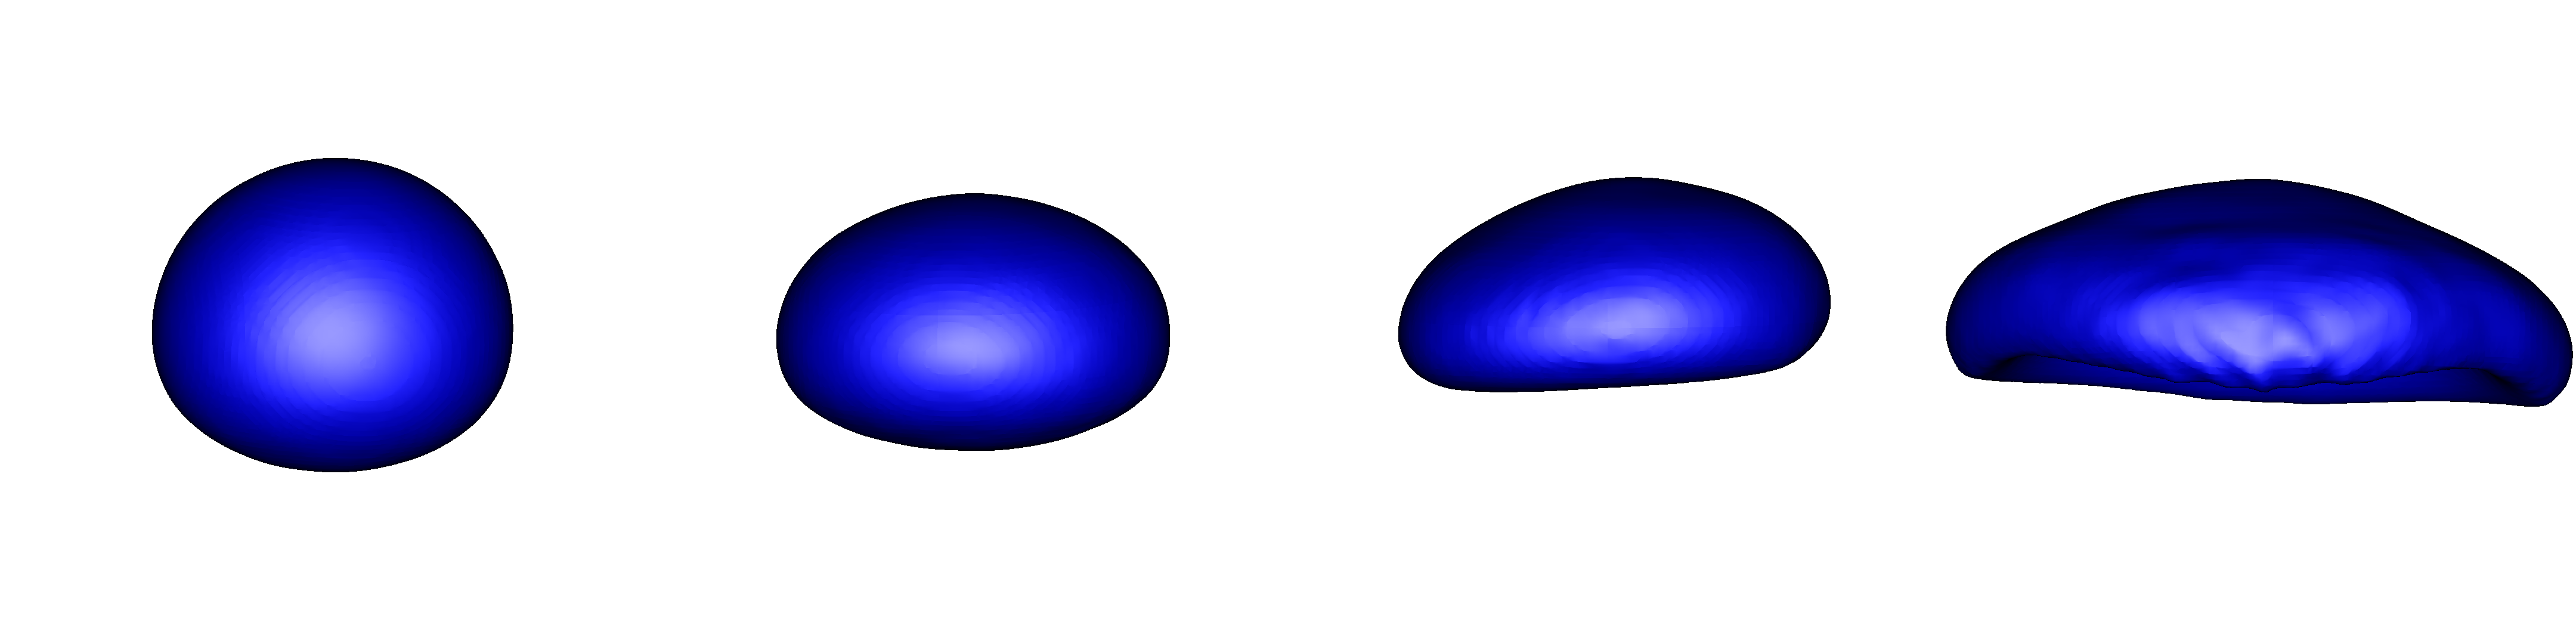
\includegraphics[width=0.99\textwidth]{Figures/flatten.png}
%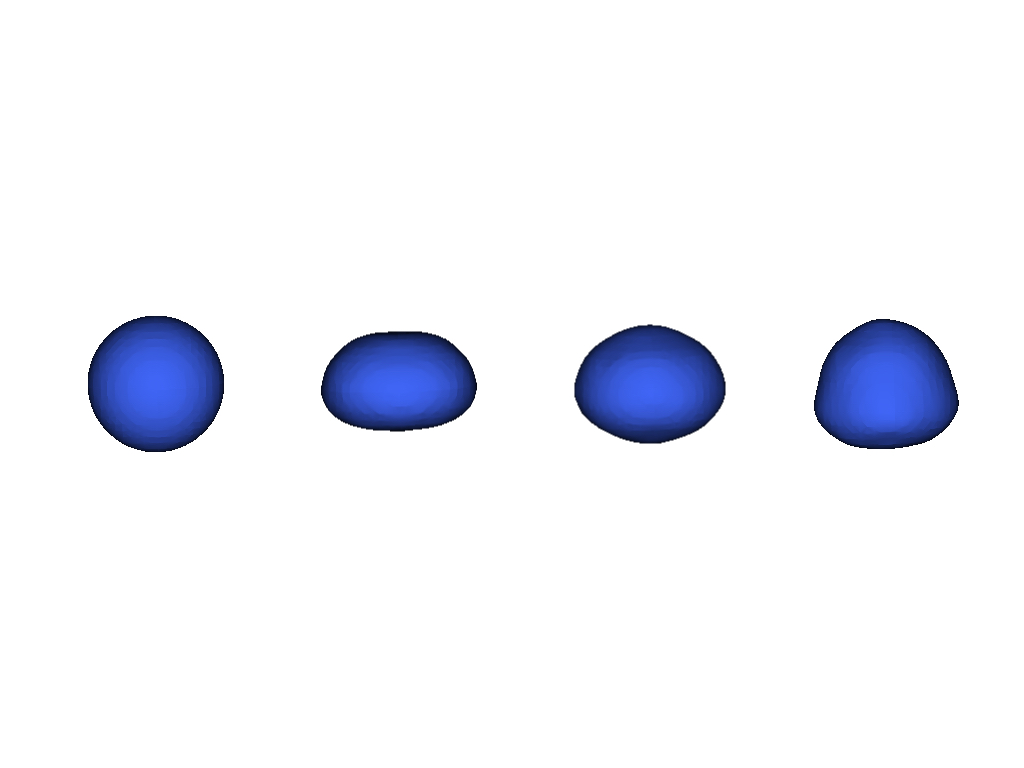
\includegraphics[width=0.99\textwidth]{Figures/Sagar/fig14-001.jpeg}
\end{center}
\caption{Flattening of the droplet with increasing equivalent diameter 
(see text). From left to right $D_e=3, \,4.6,\, 6.4$ and $8\, mm$.}
\label{flatten}
\end{figure}
% -----

From the values of the moments of inertia, the horizontal and vertical 
extents of the droplet (respectively $D_r$ and $D_x$) can be found 
and compared to the values found by the authors of \cite{Reyssat:2007ko}. 
We find $D_r=3.1 \,mm$ and $D_x=2.6 \,mm$, while ref. \cite{Reyssat:2007ko} 
concludes that drops are quasi-spherical for an equivalent diameter 
$D_e \le l_c$ and deformed for $D_e > l_c$, where $l_c =(\sigma/\rho g)^{1/2}$ 
is the capillary length, $l_c = 2.7 \,mm$ for water. 
Indeed repeating the simulations for larger drops we find increased 
flattening as shown on Figure \ref{flatten}. 

We have to keep in mind that the velocity inflow condition does not correspond to the 'exact' teminal velocity field an actual falling raindrop might experience, hence the droplet in our numerical setup does have some finite acceleration due to the imbalance between the aerodynamic forces and gravity. In Figure \ref{drop_vel}, we demonstrate the velocity of the center of mass of the droplet as a function of time, and its behavior as we increase the droplet resolution. As one can observe, due to the imbalance of forces acting on the droplet, it undergoes a net acceleration as evidenced by the approximately linear increase (absolute value) in the velocity as a function of time. The temporal variation in the droplet velocity is fitted to a linear polynomial in order to evaluate the droplet acceleration by means of a standard least-squares approach, for each droplet resolution. We illustrate (inset Figure \ref{drop_vel}) that we achieve more accurate fits as a consequence of higher droplet resolutions, as evidenced by decrease in the standard error on the fits ranging from $\pm 11.1 \%$ for $D/h = 8$ to a value of $\pm 0.12 \%$ for the highest resolution of $D/h = 64$. This provides us with an indirect indication that our numerical method can be used to generate high fidelity models of the underlying dynamics, provided sufficient resolution.           


%
%\clearpage

% Slightly less stable methods result when one takes $\hat x = x_i$. 
% In that case we observe at low resolution ($D/h=15$) the energy spike shown 
% in Figure \ref{lowres}. The energy spike is 
% associated with a moving bump on the droplet. Using a higher resolution 
% of $D/h=30$ makes the energy spike disappear. 
% Switching to the shifting of the interpolation point $\hat x$ described in 
% Section \ref{tunedinter}, even more stable behavior is observed, down 
% to resolutions of $D/h=8$. 
% -----
% \begin{figure}
% \begin{center}
% \begin{tabular}{cc}
% 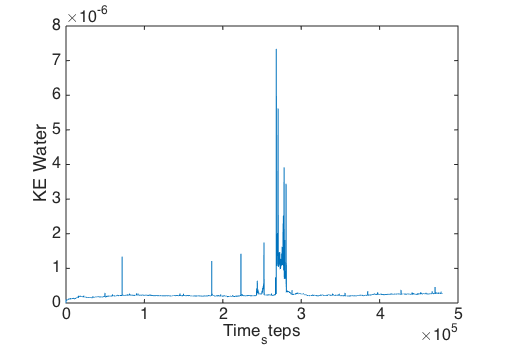
\includegraphics[width=0.5\textwidth]{Figures/KE.png}
% & 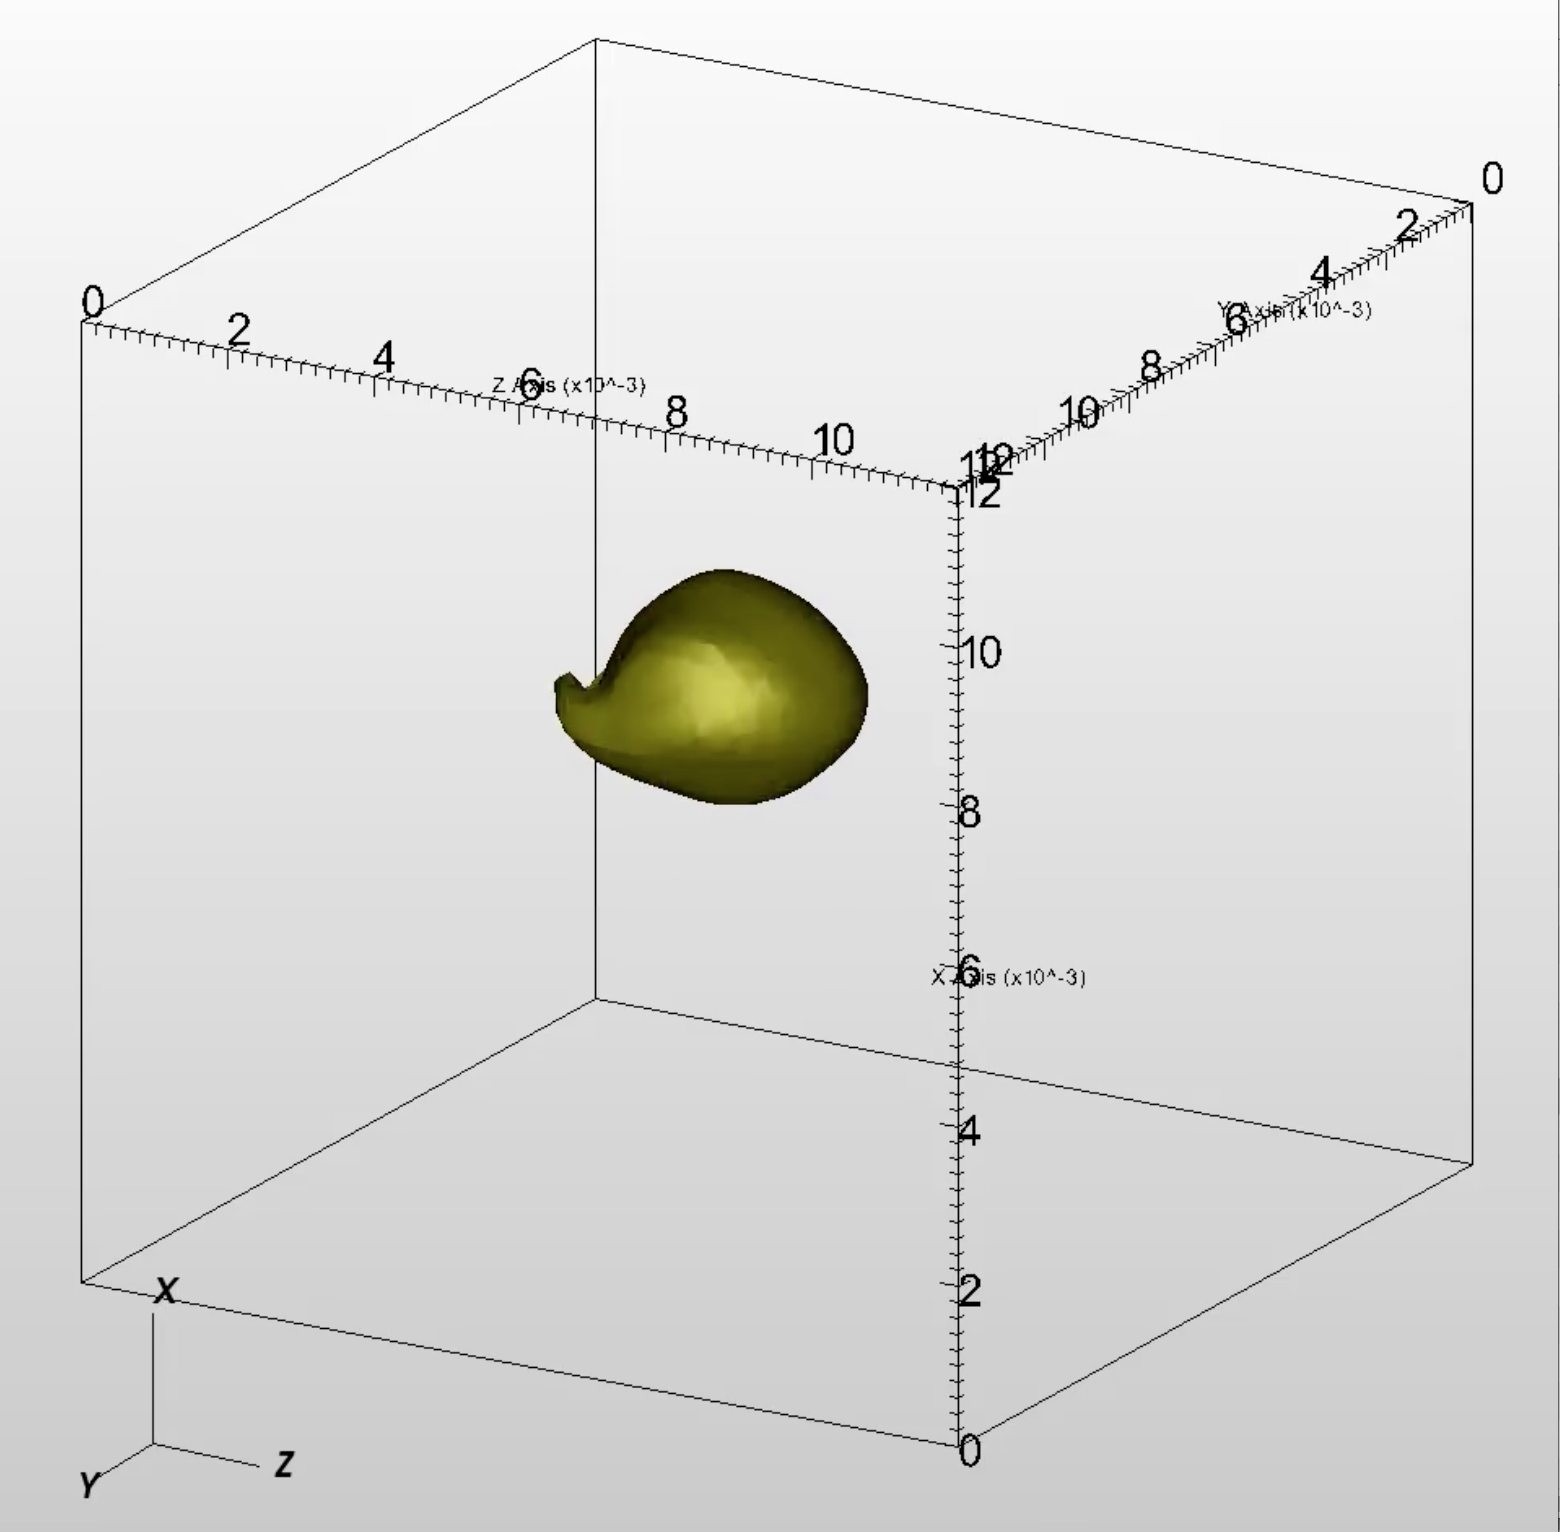
\includegraphics[width=0.4\textwidth]{Figures/bump.png} \\
% (a) & (b)
% \end{tabular}
% \end{center}
% \caption{Effect of a slightly unstable setup. (a) The kinetic energy 
% as a function of time exhibits several
% spikes (b) A snapshot of the simulation at the instant of the formation 
% of the first spike. A pointed
% bump forms on the droplet and starts rotating rapidly.}
% \label{lowres}
% \end{figure}
% -----
%% -----
%\begin{figure}
%\begin{center}
%\begin{tabular}{cc}
%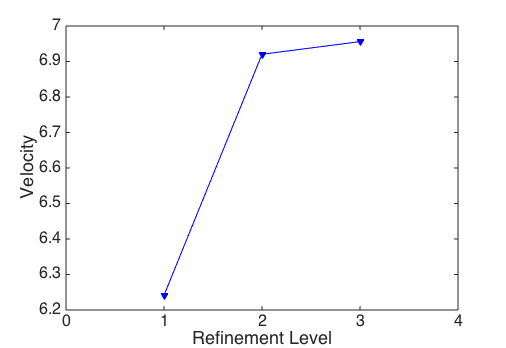
\includegraphics[width=0.45\textwidth]{Figures/veloconv.png}
%& 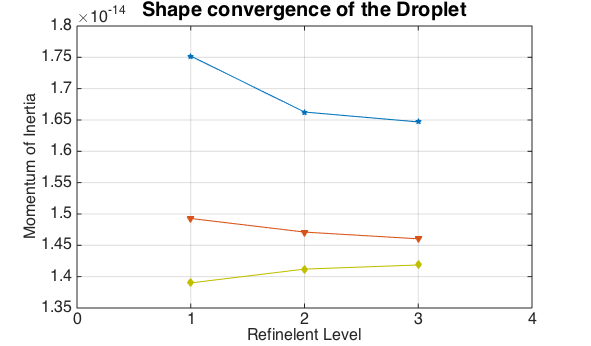
\includegraphics[width=0.45\textwidth]{Figures/shapeconv.png} \\
%(a) & (b)
%\end{tabular}
%\end{center}
%\caption{Convergence of simulations. (a) Evolution of the terminal velocity 
%with grid refinement. (b) Evolution of the three moments of inertia with 
%grid refinement.}
%\label{converge}
%\end{figure}
%% -----
% -----



\subsection{Atomizing air and water planar jets}

We also test the capability of the VOF-consistent momentum-conserving scheme 
to simulate complex air-water flows with an unstable shear flow. For that 
purpose we repeat the setup of reference \cite{Ling16}. Two jets of air and water 
are entering the computational domain from the left of Figure \ref{atom}
at velocities comparable to those of experiments. However in order to 
save computational time the domain is smaller than in experiments. Physical 
properties of air and water are identical to those of the falling raindrop case 
given in Table \ref{raindropprop}. The flow and domain characteristics are 
given in Table \ref{PhysicalParam} including a gas boundary layer 
and separator-plate size identical to those of reference \cite{Ling16}. 
The notations are as in reference \cite{Ling16}: $H_p$ is the thickness of the
jet of phase $p$, there is a separator plate of thickness $l_y$ and a 
gas boundary layer of thickness $\delta_g$.  The two streams have 
equal thickness $H_l=H_g$. The dimensionless parameters are given in 
Table \ref{dimensionlessParam}. The CIAM advection method has been used. 
The number of grid points in the layer $H_l/h = 16$ is relatively small
(compared to the  $H_l/h = 32$ in the smallest (coarsest) simulation
of reference \cite{Ling16}). It is thus all the more remarkable that the 
simulation is stable since using a smaller number of grid points usually 
increases the trend towards instability. It is interesting to note 
that the VOF calculations accounts for 31.5\% of the total time, while the 
inversion of the Poisson operator for the pressure accounted for 51.5\%. 
The whole simulations runs overnight on a present-day workstation. 

% -----
\begin{figure}
\begin{center}
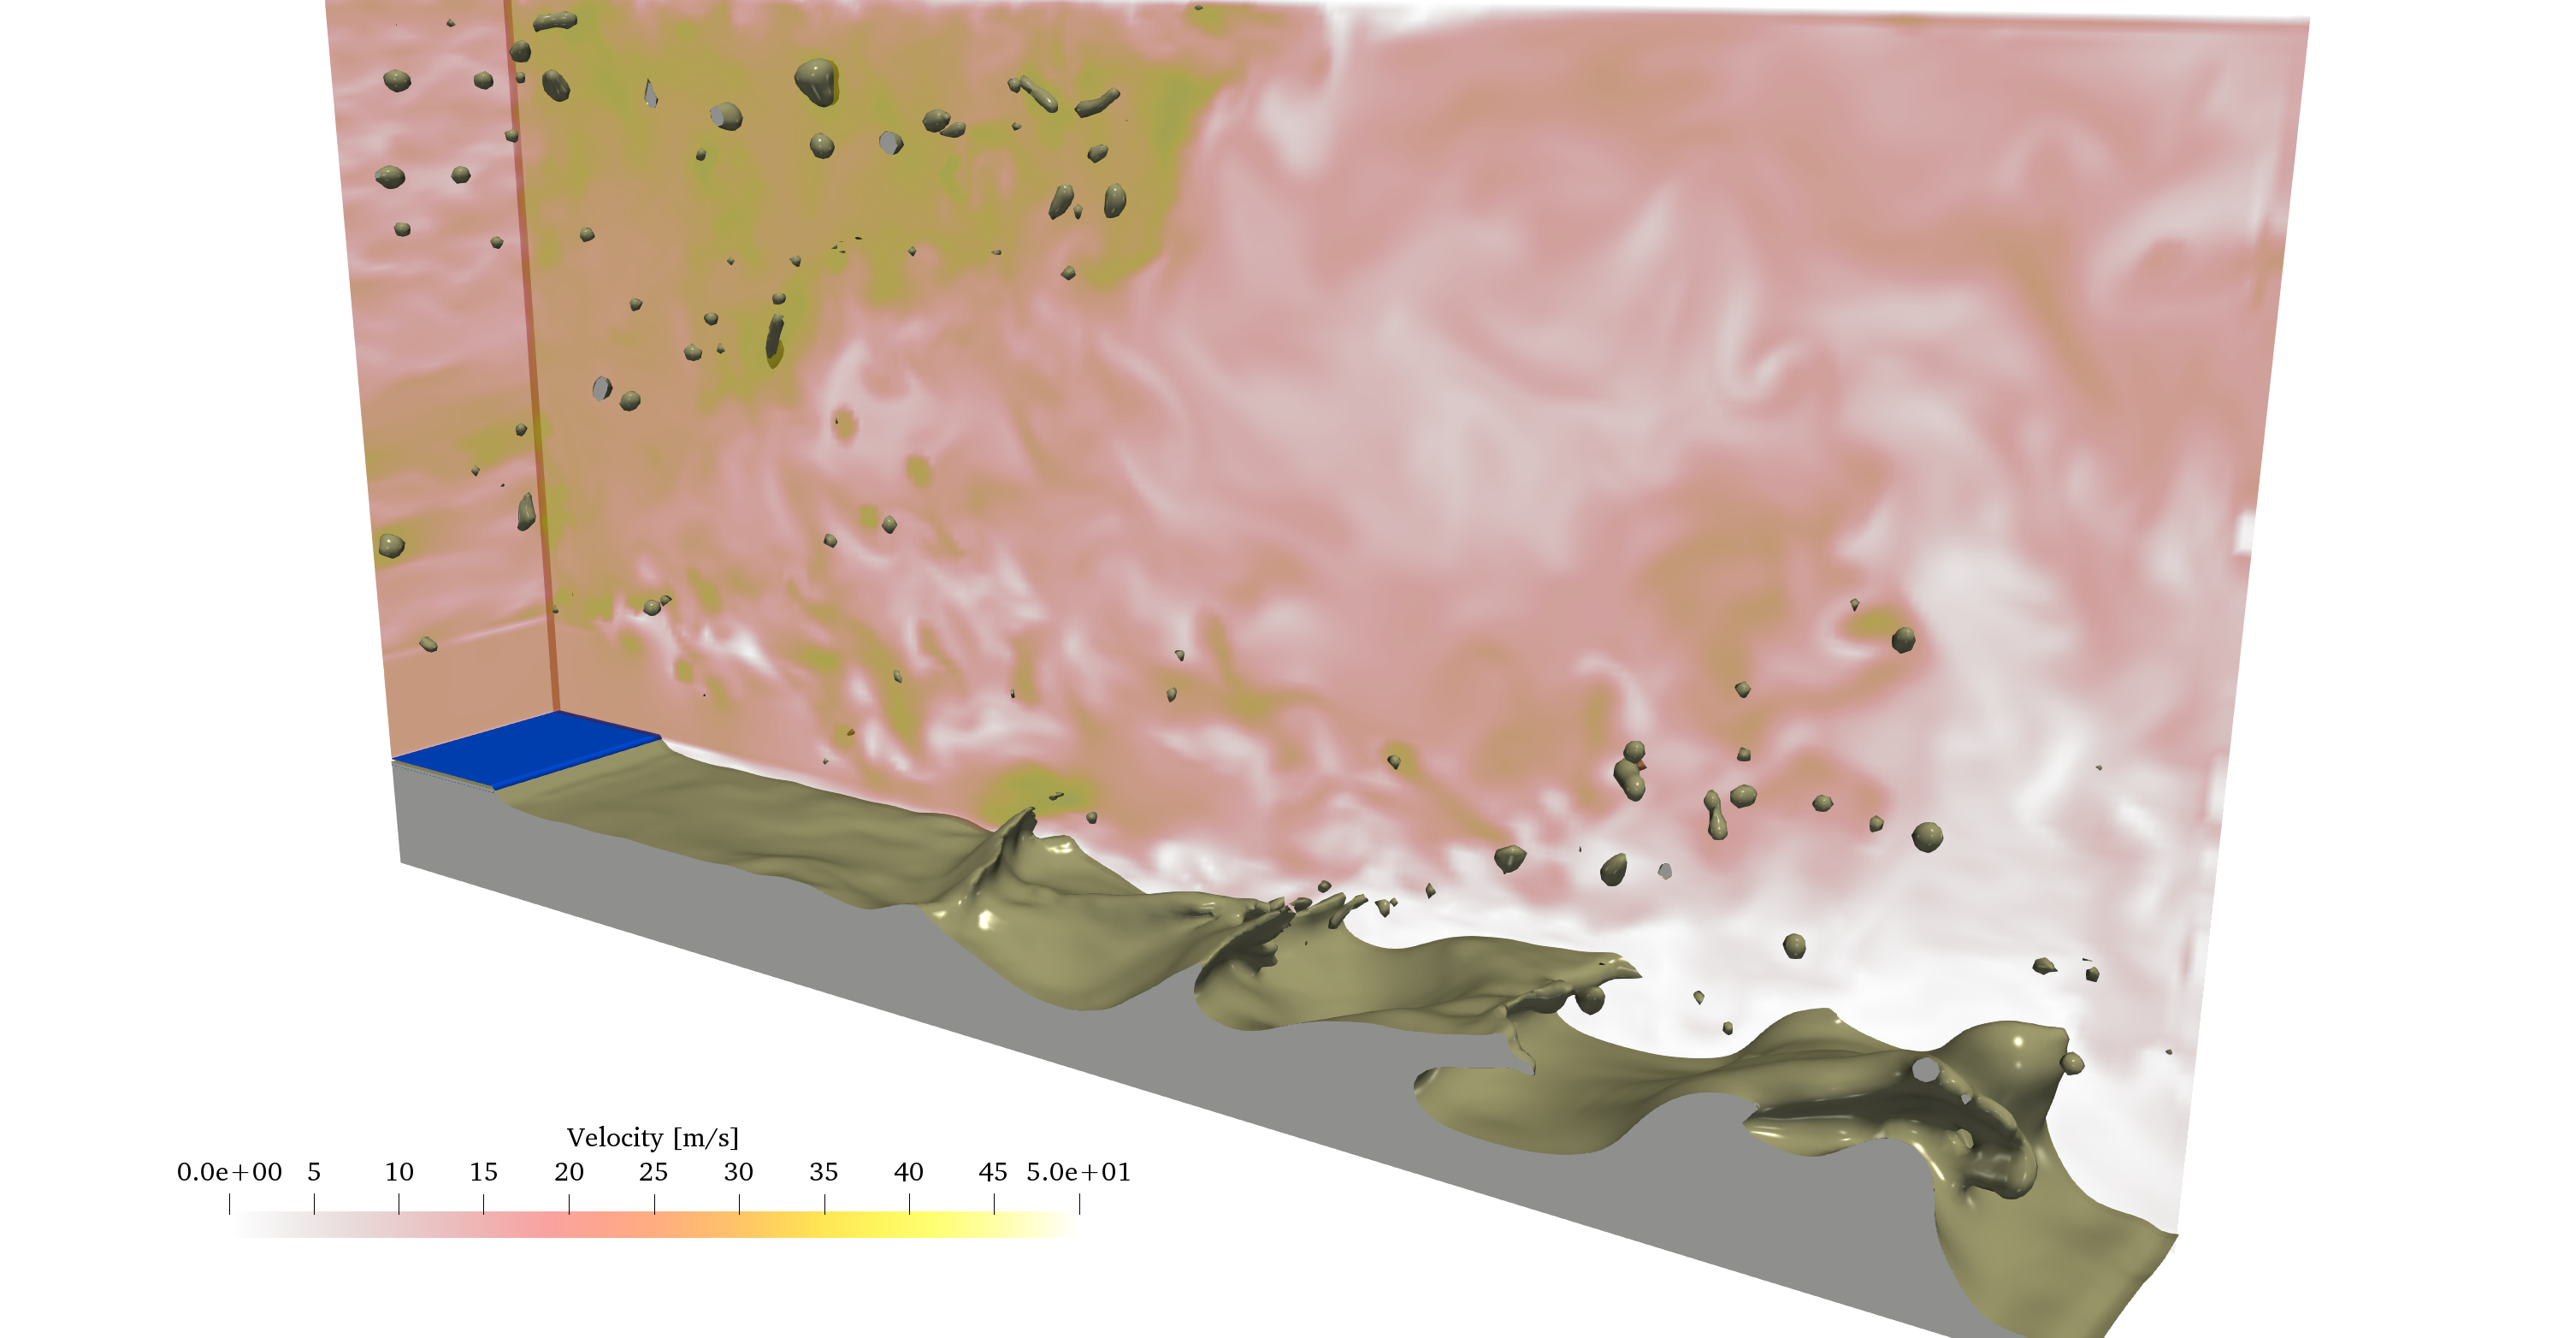
\includegraphics[width=0.99\textwidth]{Figures/Marco/vof-vel-atom.png}
\end{center}
\caption{Atomizing layer with air/water properties.}
\label{atom}
\end{figure}
% -----

% -----
\begin{table}
\begin{center}
\begin{tabular}{cccccc}
\hline
\hline
 $U_l$ & $U_g$ & $H_l$ & $h$ & $l_y$ & ${\delta_g}/{l_y}$ \\

 $(m/s)$ & $(m/s)$ & $(m)$ & $(m)$ & $(m)$ & $(-)$ \\
\hline
 $1$ & $25$ & $4\, 10^{-3}$ & $2.5\, 10^{-4}$ & $2.5\, 10^{-4}$ & $2$\\
\hline
\hline
\end{tabular}
\end{center}
\caption{Physical parameters (defined in the text) for the atomizing layer setup. The fluid 
properties are the same as in Table~\ref{raindropprop}.
}
\label{PhysicalParam}
\end{table}
% -----

% -----
\begin{table}
\begin{center}
\begin{tabular}{cccccc}
\hline
\hline
 $M$ & $r$ & $m$ & $\Re_{g,\delta}$ & $\We_{g,\delta}$  & $\Re_{g}$ \\
 $\rho_g U_g^2/\left(\rho_l U_l^2\right)$ & $\rho_l/\rho_g$ 
 & $\mu_l/\mu_g$ & $\rho_g U_g H_g/\mu_g$ & $\rho_l U_l H_l/\mu_l$ 
 & $\rho_g U_g^2 H_g/\sigma$ \\
\hline
 $0.75$ & $831.8$ & $45$ & $757.6$ & $5.151$ & $6061$  \\
\hline
\hline
\end{tabular}
\end{center}
\caption{Dimensionless parameters for the atomizing layer setup.}
\label{dimensionlessParam}
\end{table}
% -----
